\documentclass[11pt, a4paper]{article}
\usepackage[utf8]{inputenc}
\usepackage[margin=.7in]{geometry}
\usepackage{listings}
\usepackage{setspace}
\usepackage{xcolor}
\usepackage{titlesec}
\usepackage{enumitem}
\usepackage{amssymb}
\usepackage{amsmath}
\usepackage{bm}
\usepackage{multicol}
\usepackage{graphicx}
\graphicspath{{./Figures/}}
\usepackage{color}
\usepackage{hyperref}
\hypersetup{
	colorlinks=true,
	linkcolor=blue,
	urlcolor=blue,
}
\titleformat*{\section}{\LARGE\bfseries\filcenter}
\titleformat*{\subsection}{\Large\bfseries}
\titleformat*{\subsubsection}{\large\bfseries}
\definecolor{codegreen}{rgb}{0,0.5,0}
\definecolor{codegray}{rgb}{0.5,0.5,0.5}
\definecolor{codered}{rgb}{0.78,0,0}
\definecolor{codepurple}{rgb}{0.58,0,0.68}
\definecolor{backcolour}{rgb}{0.95,0.95,0.92}
\lstdefinestyle{mystyle}{
    backgroundcolor=\color{backcolour},   
    commentstyle=\color{gray},
    keywordstyle=\color{codegreen},
    numberstyle=\tiny\color{codegray},
    stringstyle=\color{codered},
    basicstyle=\ttfamily\footnotesize,
    breakatwhitespace=false,         
    breaklines=true,                 
    captionpos=b,                    
    keepspaces=true,                 
    numbers=left,                    
    numbersep=5pt,                  
    showspaces=false,                
    showstringspaces=false,
    showtabs=false,                  
    tabsize=2,
    morekeywords = {as},
    keywordstyle = \color{codegreen}
}
\lstset{style=mystyle}

\begin{document}
	\begin{titlepage}
		\begin{center} \Huge \textbf{Data Science} \end{center}
		\tableofcontents
		\newpage
	\end{titlepage}
%%%% PAGE 1 %%%%
	\begin{spacing}{1.1}
	\section{Introduction to SQL}
	\subsection{Relational Database Management System}
	A \textbf{database} is a set of data stored in a computer. This data is usually structured in a way that makes the data easily accessible. A \textbf{relational database} is a type of database. It uses a structure that allows us to identify and access data in \textit{relation} to another piece of data in the database. Often, data in a relational database is organized into tables with records (rows) and columns. \vspace*{1mm}\\
	A \textbf{relational database management system (RDBMS)} is a program that allows you to create, update, and administer a relational database. Most use SQL language to access the database. However, SQL syntax can differ based on  which RDBMS you are using. \\
	
	\subsection{Data Manipulation in SQL}
	- A statement always ends in a semicolon \textbf{;} \vspace*{1mm}\\
	Components of a statement: \\
	1) Clause -  perform specific task is SQL, written in capital letters (known as commands) \\
	2) Table name - written in lowercase letters, name of table to apply command to \\
	3) Parameters - list of columns, data types, or values that are passed to a clause as an argument\\~\\
	The \textbf{CREATE} statement allows use to create a new table in the database 
	\begin{lstlisting}[language=SQL]
	CREATE TABLE table_name (
		column1 datatype,
		column2 datatype,
		column3 datatype
	);	\end{lstlisting} \vspace*{1mm}
	The \textbf{INSERT} and \textbf{VALUES} statements allows us to add new records (rows) to a table
	\begin{lstlisting}[language=SQL]
	-- Insert into columns in order:
	INSERT INTO table_name
	VALUES (value1, value2);
	
	-- Insert into columns by name:
	INSERT INTO table_name (column1, column2)
	VALUES (value1, value2);	\end{lstlisting} \vspace*{1mm}
	The \textbf{SELECT} statements will fetch data from a database (query data from database)
	\begin{lstlisting}[language=SQL]
	SELECT column_name FROM table_name;
	SELECT * FROM tabe_name; -- all columns from table \end{lstlisting} \vspace*{1mm}
	The \textbf{ALTER TABLE} adds a new column(s) to the table (will be initialized to NULL ($\emptyset$))
	\begin{lstlisting}[language=SQL]
	ALTER TABLE table_name
	ADD column_name datatype; \end{lstlisting} \vspace*{1mm}
	The \textbf{UPDATE} statement allows use to edit existing records
	\begin{lstlisting}[language=SQL]
	UPDATE table_name
	SET column1 = value1, column2 = value2
	WHERE some_column = some_value; \end{lstlisting} \vspace*{1mm}
	The \textbf{DELETE FROM} statement deletes one or more rows from a table
	\begin{lstlisting}[language=SQL]
	DELETE FROM table_name
	WHERE some_column = some_value; \end{lstlisting} \newpage
%%%% PAGE 2 %%%%
	\noindent \textbf{Constraints} add information about how a column can be used are invoked after specifying the data type for a column. They can be used to tell the database to reject inserted data that does not adhere to a certain restriction. \\
	\hspace*{3mm} - PRIMARY KEY columns uniquely identify a row, only one per table \\
	\hspace*{3mm} - UNIQUE columns have different value for every row, can be multiple per table \\
	\hspace*{3mm} - NOT NULL columns must have a value \\
	\hspace*{3mm} - DEFAULT columns will pass an assumed value if non specified
	\begin{lstlisting}[language=SQL]
	CREATE TABLE student (
		id INTEGER PRIMARY KEY, -- Can't add another row called ID or any of the values
		name TEXT UNIQUE, -- Can't add same value in name row
		grade INTEGER NOT NULL, -- Can't leave value NULL when adding new grade
		age INTEGER DEFAULT 10 -- Passes given parameter if non given
	); \end{lstlisting} \vspace*{5mm}
	
	\subsection{Writing Queries}
	\textbf{Queries} allow us to communicate with the database by asking questions and having the result set return data relevant to the question. One of the core purposes of the SQL language is to retrieve information stored in a database. \\~\\
	The \textbf{SELECT} statement is used to query data from a database, with \textbf{*} meaning all columns 
	\begin{lstlisting}[language=SQL]
	SELECT column1, column2 
	FROM table_name; \end{lstlisting} \vspace*{1mm}
	The \textbf{AS} keyword lets you rename a column or table using an specified alias. However, this doesn't rename the column in the table, only the results outputted
	\begin{lstlisting}[language=SQL]
	SELECT column_name AS 'alias'
	FROM table_name; \end{lstlisting} \vspace*{1mm}
	The \textbf{DISTINCT} keyword allows us to return only unique values in the output, filtering all duplicates
	\begin{lstlisting}[language=SQL]
	SELECT DISTINCT column_name 
	FROM table_name; \end{lstlisting} \vspace*{1mm}
	The \textbf{WHERE} clause lets us restrict our query results where a condition is true ($=,!=,<,>,<=,>=$)
	\begin{lstlisting}[language=SQL]
	SELECT column_name 
	FROM table_name 
	WHERE condition; \end{lstlisting} \vspace*{1mm}
	The \textbf{LIKE} is a special operator used with WHERE to search for a specific pattern in a column \\
	\hspace*{3mm} - The \_ wildcard means substitute any character\\
	\hspace*{3mm} - The \% wildcard means matching zero or more missing letters in the pattern (not case sensitive)
	\begin{lstlisting}[language=SQL]
	SELECT * 
	FROM movies
	WHERE name LIKE 'Se_en'; -- The _ means any character (return 'Seven' and 'Se7en')
	-- WHERE name LIKE 'A%' matches all movies beginning with letter A
	-- WHERE name LIKE '%a' matches all movies end with letter a
	-- WHERE name LIKE '%man%' matches all movies containing 'man' \end{lstlisting} \vspace*{1mm}
	We can test for NULL values with operates \textbf{IS NULL} and \textbf{IS NOT NULL} (can't use = or !=)
	\begin{lstlisting}[language=SQL]
	SELECT column_name
	FROM table_name 
	WHERE column_name IS NULL; -- or IS NOT NULL \end{lstlisting} \vspace*{1mm}
%%%% PAGE 3 %%%%
	The \textbf{BETWEEN} operator is used with WHERE to filter results within a certain range \\
	\hspace*{3mm} - Number ranges include the final value (ex: 1970 AND 1979 includes 1979) \\
	\hspace*{3mm} - Text ranges do not include final value (ex: `A' AND `D' stops before D)
	\begin{lstlisting}[language=SQL]
	SELECT *
	FROM movies
	WHERE year BETWEEN 1990 AND 1999; -- includes 1999
	-- WHERE name BETWEEN 'A' AND 'J'; up to, but not including, J \end{lstlisting} \vspace*{1mm}
	The \textbf{AND} or \textbf{OR} operators to combine multiple conditions in a WHERE clause
	\begin{lstlisting}[language=SQL]
	SELECT * 
	FROM movies
	WHERE year BETWEEN 1990 AND 1999
		AND genre = 'romance'; -- both conditions must be true 
	
	SELECT *
	FROM movies
	WHERE year > 2014 OR genre = 'action'; -- either condition is true \end{lstlisting}  \vspace*{1mm}
	\noindent The \textbf{ORDER BY} lets ys sort results (alphabetic or numeric). We can pass the given keywords: \\
	\hspace*{3mm} - DESC to sort results descending (high-low or Z-A) \\
	\hspace*{3mm} - ASC to sort results ascending (low-high or A-Z) \\
	NOTE: If a WHERE clause is present, the ORDER BY goes after
	\begin{lstlisting}[language=SQL]
	SELECT column_name
	FROM table_name
	ORDER BY column_name DESC; -- can also be ASC (ASC is same as blank) \end{lstlisting} \vspace*{1mm}
	The \textbf{LIMIT} clause lets you specify the max number of rows the result set will have (at end of query)
	\begin{lstlisting}[language=SQL]
	SELECT column_name
	FROM table_name
	LIMIT num_value; -- replace num_value with an integer \end{lstlisting} \vspace*{1mm}
	The \textbf{CASE} statement allows us to create different outputs (SQL's if-then logic). Each WHEN tests a condition and if true, executes the THEN parameter. ELSE parameter is executed if all WHEN tests are false. Always finish CASE statement with END.
	\begin{lstlisting}[language=SQL]
	SELECT name, -- given column name
		CASE
			WHEN genre = 'romance' THEN 'Chill' -- If romance genre then label chill
			WHEN genre = 'comedy' THEN 'Chill' -- if comedy then label chill
			ELSE 'Intense' -- if both above false, then label intense
		END AS 'Mood' -- label column with all results
	FROM movies; -- table to read from \end{lstlisting} \vspace*{5mm}
		
	\subsection{Aggregate Functions}
	We will know learn about \textbf{aggregates} which are calculations performed on multiple rows of a table. \\~\\
	The \textbf{COUNT()} function returns the total number of rows that match the specified criteria (excludes $\emptyset$)
	\begin{lstlisting}[language=SQL]
	SELECT COUNT(column_name) -- can be *
	FROM table_name
	WHERE condition; -- this line is optional \end{lstlisting} \newpage
%%%% PAGE 4 %%%%
	\noindent The \textbf{SUM()} function takes a column name as an argument and returns sum of all values in column.
	\begin{lstlisting}[language=SQL]
	SELECT SUM(column_name)
	FROM table_name; \end{lstlisting} \vspace*{1mm}
	The \textbf{MAX()} and \textbf{MIN()} functions return the highest and lowest values in a column, respectively.
	\begin{lstlisting}[language=SQL]
	SELECT MAX(column_name) -- can also be MIN(column_name)
	FROM table_name; \end{lstlisting} \vspace*{1mm}
	The \textbf{AVG()} function to quickly calculate the average value of a particular column
	\begin{lstlisting}[language=SQL]
	SELECT AVG(column_name)
	FROM table_name; \end{lstlisting} \vspace*{1mm}
	The \textbf{ROUND()} function takes two parameter, a column name and an integer, and rounds the result
	\begin{lstlisting}[language=SQL]
	SELECT ROUND(column_name, integer)
	FROM table_name; \end{lstlisting} \vspace*{1mm}
	The \textbf{GROUP BY} function arranges identical data into groups (NOTE: comes after FROM or WHERE, but before ORDER BY or LIMIT). We can also use GROUP BY on columns by using integers instead of strings (1 = first column select, 2 = second column selected, ...)
	\begin{lstlisting}[language=SQL]
	SELECT price, COUNT(*) -- shows price and count all rows
	FROM fake_apps
	WHERE downloads > 20000 -- where over 20000 downloads
	GROUP BY price; -- sort results by price 
	
	SELECT category, price, AVG(downloads)
	FROM fake_apps
	GROUP BY 1, 2; -- groups by category and price \end{lstlisting} \vspace*{1mm}
	The \textbf{HAVING} function filters groups for a query built with aggregate properties (similar to WHERE)\\
	NOTE: HAVING always comes after GROUP BY but before ORDER BY and LIMIT
	\begin{lstlisting}[language=SQL]
	SELECT price, ROUND(AVG(downloads)), COUNT(*)
	FROM fake_apps
	GROUP BY price -- group by price
	HAVING COUNT(name) > 10; -- filter groups where they must have 10+ apps \end{lstlisting} \vspace*{1mm}
	The \textbf{strftime()} function takes two parameters, the format a column name \\
	\hspace*{3mm} - Formats: Click \href{https://www.sqlite.org/lang_datefunc.html}{this} link to see all the format options
	\begin{lstlisting}[language=SQL]
	SELECT timestamp,
	strftime('%H', timestamp) -- returns the hour of our timestamp column
	FROM hacker_news
	GROUP BY 1
	LIMIT 20; \end{lstlisting} \vspace*{1mm}
	FROM `THE MET' PROJECT
	\begin{lstlisting}[language=SQL]
	SELECT CASE
		WHEN medium LIKE '%gold%'   THEN 'Gold' -- any art piece with gold in name
		WHEN medium LIKE '%silver%' THEN 'Silver' -- any art piece with silver in name
		ELSE NULL -- all other art pieces are NULL
	 END AS 'Bling', -- rename results column as Bling
	 COUNT(*) -- part of select statement to count all rows
	FROM met
	WHERE Bling IS NOT NULL -- discard all non gold/silver pieces
	GROUP BY 1 -- group by CASE column
	ORDER BY 2 DESC; -- order by number of items (COUNT) \end{lstlisting} \newpage
%%%% PAGE 5 %%%%
	\subsection{Multiple Tables}
	In order to efficiently store data, we often spread related information across multiple tables. \vspace*{2mm}\\
	The \textbf{JOIN} function lets us combine tables easily. This simple JOIN is called an \textit{inner join}, and will only include rows that have matching values, but will omit any rows not matching our ON condition.
	\begin{lstlisting}[language=SQL]
	SELECT * -- all columns
	FROM orders -- from orders table
	JOIN subscriptions -- joined with subscriptions table
		ON orders.subscription_id = subscriptions.subscription_id -- match these columns
	WHERE subscriptions.description = 'Fashion Magazine'; -- only for this description \end{lstlisting} \vspace*{1mm}
	The \textbf{LEFT JOIN} allows us to combine two tables and keep the unmatched rows we would lose in the inner join (keeps all values from the left table in the FROM statement and fills in missing values in the right table with NULL values)
	\begin{lstlisting}[language=SQL]
	SELECT * -- select all columns
	FROM newspaper -- keep all rows from newspaper table
	LEFT JOIN online -- join with online table
		ON newspaper.id = online.id -- match these columns
	WHERE online.id IS NULL; -- see who subscribes to newspaper but not online \end{lstlisting} \vspace*{1mm}
	A \textbf{Primary Key} is a column that uniquely identifies each row of a table. They have a few requirements: \\
	\hspace*{3mm} - None of the values can be NULL \\
	\hspace*{3mm} - Each value is unique (no 2 rows with same value) \\
	\hspace*{3mm} - A table can only have one primary key column \\
	Now, when a primary key for one table appears in a different table, it is a \textbf{Foreign Key}. This is important because the most common types of joins will be joining a foreign key from one table to the primary key from another table.
	\begin{lstlisting}[language=SQL]
	SELECT * 
	FROM classes -- primary key = id
	JOIN students -- primary key = id, foreign_key = class id 
		ON classes.id = students.class_id; -- join primary key with foreign key \end{lstlisting} \vspace*{1mm}
	The \textbf{CROSS JOIN} lets all combine all rows of one table with all rows of another table (think of as finding all possible combinations of the two tables).
	\begin{lstlisting}[language=SQL]
	SELECT month, COUNT(*) AS 'subscribers' -- columns to display
	FROM newspaper -- table 1
	CROSS JOIN months -- table 2
	WHERE start_month <= month AND end_month >= month -- where user was subscribed
	GROUP BY month; -- group together results by month \end{lstlisting}\vspace*{1mm}
	The \textbf{UNION} operator lets us stack data sets on top of one another, given that thy have the same number of columns and the columns have the same data types.
	\begin{lstlisting}[language=SQL]
	SELECT *
	FROM table_name1
	UNION
	SELECT * 
	FROM table_name2; -- will put table_name2 below table_name1 \end{lstlisting} \newpage
%%%% PAGE 6 %%%%
	\noindent The \textbf{WITH} clause allows us to perform a separate query and store it in a temporary table that we can reference any columns from. We can then join this temporary table with another table
	\begin{lstlisting}[language=SQL]
	WITH previous_query AS ( -- create a temp table
		SELECT customer_id, COUNT(subscription_id) AS 'subscriptions' -- select columns
		FROM orders -- table
		GROUP BY customer_id -- grouped by customer id
	) -- end of our temp table query
	SELECT customers.customer_name, previous_query.subscriptions -- new col., temp col.
	from previous_query -- from temp table
	JOIN customers -- inner join with cutomers table
		ON previous_query.customer_id = customers.customer_id; -- if parameters met \end{lstlisting} \vspace*{4mm}
		
	\subsection{Usage Funnels}
	A \textbf{funnel} is a marketing model which illustrates the theoretical customer journey towards the purchase of a product or service. Oftentimes, we want to track how many users complete a series of steps and know which steps have the most number of users giving up. \\~\\
	We can \textbf{build a funnel from a single table}. Lets count the distinct users who answered each question.
	\begin{lstlisting}[language=SQL]
	SELECT question_text, COUNT(DISTINCT user_id)
	FROM survey_responses
	GROUP BY 1; \end{lstlisting}\vspace*{1mm}
	We can \textbf{compare funnels for A/B tests}. Half of the users view the original control version and half view the new variant version, lets count the control and variant clicks for each modal step
	\begin{lstlisting}[language=SQL]
	SELECT modal_text, 
		COUNT(DISTINCT CASE
			WHEN ab_group = 'control' THEN user_id
			END) AS 'control_clicks', -- creat column for control clicks
		COUNT(DISTINCT CASE
			WHEN ab_group = 'variant' THEN user_id
			END) AS 'variant_clicks' -- create column for version clicks
	FROM onboarding_modals
	GROUP BY 1
	ORDER BY 1; \end{lstlisting}\vspace*{1mm}
	We can also \textbf{build a funnel from multiple tables}. In the end, we want to see if the conversion rate from checkout to purchase changes as we get closer to Christmas.
	\begin{lstlisting}[language=SQL]
	WITH funnels AS (
		SELECT DISTINCT b.browse_date, -- distinct browse dates
			b.user_id, -- get all user id's
			c.user_id IS NOT NULL AS 'is_checkout', -- 1 if in checkout, 0 if not
			p.user_id IS NOT NULL AS 'is_purchase' -- 1 if purchased, 0 if not
		FROM browse AS 'b' -- rename table browse as b
		LEFT JOIN checkout AS 'c' -- join c with b
			ON c.user_id = b.user_id -- match c user id to b user id
		LEFT JOIN purchase AS 'p' -- join p with bc table
			ON p.user_id = c.user_id) -- match p user id to bc table user id
	SELECT browse_date, COUNT(*) AS 'num_browse', -- browse dates, users in browse stage
		SUM(is_checkout) AS 'num_checkout', -- total number in checkout stage
		SUM(is_purchase) AS 'num_purchase', -- total numberin  purchased stage
		1.0 * SUM(is_checkout) / COUNT(user_id) AS 'browse_to_checkout', -- b:c ratio
		1.0 * SUM(is_purchase) / SUM(is_checkout) AS 'checkout_to_purchase' -- c:p ratio
	FROM funnels -- from temp table
	GROUP BY 1 -- group by browse date
	ORDER BY 1; -- order by browse date (ASC) \end{lstlisting} \newpage
%%%% PAGE 7 %%%%
	\noindent USAGE FUNNELS WITH WARBY PARKER PROJECT 
	\begin{lstlisting}[language=SQL]
	WITH temp_results AS ( -- create temp table
		SELECT DISTINCT q.user_id, 
			ht.user_id IS NOT NULL AS 'is_home_try_on', -- 0 if no glasses, 1 if has glasses
			ht.number_of_pairs, -- 3 pairs, 5 pairs (A/B testing)
			p.user_id IS NOT NULL as 'is_purchase' -- 0 if no purchase, 1 if purchase
		FROM quiz q -- quiz table referenced as q
		LEFT JOIN home_try_on ht 
			ON q.user_id = ht.user_id -- where user id's match
		LEFT JOIN purchase p
			ON q.user_id = p.user_id -- where user id's match
		WHERE ht.number_of_pairs IS NOT NULL ) -- customer has either A/B test
	SELECT number_of_pairs AS 'Try On Pairs', -- 3 or 4 pairs 
		COUNT(*) AS 'Customers', -- total for customers
		SUM(is_purchase) AS 'Purchased Product', -- if customer bought product
		1.0 * SUM(is_purchase) / COUNT(*) AS 'Purchase Rate' -- rate of purchase
	FROM temp_results -- from temp table above
	GROUP BY 1 -- group by pair type
	ORDER BY 4 DESC; -- order by purchase rate 
	-- We see that 5 pairs purchase rate = 79%, 3 pairs purchase rate = 53% \end{lstlisting}\vspace*{4mm}
	
	\subsection{User Churn}
	\textbf{Churn rate} is the percent of subscribers that have canceled within a certain period, usually a month. For a user base to grow, the churn rate must be less than the new subscriber rate for the same period and is calculated by $\frac{cancellations}{total\;subscribers}$.\\~\\
	We can calculate churn for a month from a single table 
	\begin{lstlisting}[language=SQL]
	SELECT 1.0 * (
		SELECT COUNT(*)
		FROM subscriptions
		WHERE subscription_start < '2017-01-01' 
		AND (subscription_end BETWEEN '2017-01-01' AND '2017-01-31')
	 ) / (
		SELECT COUNT(*)
		FROM subscriptions
		WHERE subscription_start < '2017-01-01'
		AND ((subscription_end >= '2017-01-01') 
			OR (subscription_end IS NULL))
	) AS results; \end{lstlisting}\newpage
	
	
	\section{Introduction to Python}
	\subsection{Lists}
	We can use \textbf{zip()} to create pairs from multiple lists. However, it returns the location in memory and must be converted back to a \textbf{list()} in order to print it.\\ 
	We can add a single element to a list using \textbf{.append()}, which will place at the end of the list. \\
	We can add multiple lists together by using $\bm{+}$ to concatenate them.
	\begin{lstlisting}[language=Python]
	last_semester_gradebook = [("politics", 80), ("latin", 96), ("dance", 97), 
	                           ("architecture", 65)]
	
	subjects = ["physics", "calculus", "poetry", "history"]
	grades = [98, 97, 85, 88]
	subjects.append("computer science")
	grades.append(100)
	gradebook = list(zip(subjects,grades)) # combine and cast as a list
	gradebook.append(("visual arts", 93)) # append a tuple
	print(gradebook)
	
	full_gradebook = gradebook + last_semester_gradebook
	print(full_gradebook) \end{lstlisting}\vspace*{1mm}
	We can create an array of integers for a given size by \textbf{range()}, which generates starting at a point (0 by default) to the (input value - 1). However, you must convert it to a list since it returns on object.
	\begin{lstlisting}[language=Python]
	my_list = range(9) # values 0 to 8
	my_list_2 = range(5, 15, 3) # start at 5, end at 14, increment by 3
	print(list(my_list_2)) # [5, 8, 11, 14] \end{lstlisting}\vspace*{1mm}
	We can select a section of a list by using syntax array[start:stop], called \textbf{slicing}. 
	\begin{lstlisting}[language=Python]
	suitcase = ['shirt', 'shirt', 'pants', 'pants', 'pajamas', 'books']
	start = suitcase[:3] # same as suitcase[0:3]
	end = suitcase[-2:] # gets last 2 elements of suitcase \end{lstlisting}\vspace*{1mm}
	We can count how many times an element appears in a list with \textbf{.count()}
	\begin{lstlisting}[language=Python]
	votes = ['Jake', 'Jake', 'Laurie', 'Laurie', 'Laurie', 'Jake']
	jake_votes = votes.count('Jake')
	print(jake_votes) \end{lstlisting}\vspace*{1mm}
	We can sort a list alphabetically or numerically with \textbf{.sort()} - only alters a list, doesn't return a value \\
	We can use \textbf{sorted()} to also sort a list, but it will not affect the original list (returns sorted copy)
	\begin{lstlisting}[language=Python]
	games = ['Portal', 'Minecraft', 'Pacman', 'Tetris', 'The Sims', 'Pokemon']
	
	games_sorted = sorted(games)
	print(games) # in same order as above
	print(games_sorted) # new list of sorted games
	
	games.sort()
	print(games) # now the games list is also sorted \end{lstlisting}\vspace*{1mm}
	\textbf{Tuples} are immutable (can't change any values after creating) and are denoted with ( ) \\
	We use tuples to store data that belongs together and don't need order or size to change
	\begin{lstlisting}[language=Python]
	my_info = ('Derek', 22, 'Student')
	name, age, occupation = my_info # will assign each value to a varaible
	
	one_element_tuple = (4,) # NOTE: we need the , after 4 otherwise it wont be a tuple
	one_element_tuple_2 = (4) # same as one_element_tuple_2 = 4	 \end{lstlisting} \newpage
%%%% PAGE 9 %%%%
	
	\subsection{Loops}
	We can use \textbf{for} loops to iterate through each item in a list, with the following general formula \\
	\hspace*{3mm} - We can use range() to execute a for loop from start (0 by default) to stop (n-1) \\
	\hspace*{3mm} - We can use \textit{break} to exit a for loop when a certain value is found \\
	\hspace*{3mm} - We can use \textit{continue} to move to the next index in a list if a condition is found \\
	If we have a list made of multiple lists, we use \textbf{nested} loops to iterate through them
	\begin{lstlisting}[language=Python]
	sales_data = [[12, 17, 22], [2, 10, 3], [5, 12, 13]]
	scoops_sold = 0
	
	for location in sales_data: # for each list in list
		for sales in location: # for each element in inner list
			scoops_sold += sales
	
	print(scoops_sold) \end{lstlisting}\vspace*{1mm}
	We can use \textbf{list comprehension} to efficiently iterate through a list instead of a for loop \\
	We can also use this to alter values in a list and create a new list
	\begin{lstlisting}[language=Python]
	heights = [161, 164, 156, 144, 158, 170, 163, 163, 157] # in cm's
	
	can_ride_coaster = [cm for cm in heights if cm > 161]
	print(can_ride_coaster) # [164, 170, 163, 163] 
	
	celsius = [0, 10, 15, 32, -5, 27, 3] # degrees in C
	
	fahrenheit = [f_temp * (9/5) + 32 for f_temp in celsius] # convert C to F degrees
	print(fahrenheit) # [32.0, 50.0, 59.0, 89.6, 23.0, 80.6, 37.4] \end{lstlisting}\vspace*{4mm}
	
	\subsection{List Comprehension / Lambda Functions}
	We can iterate through lists within lists with the following syntax
	\begin{lstlisting}[language=Python]
	nested_lists = [[4, 8], [15, 16], [23, 42]]
	
	product = [(val1 * val2) for (val1, val2) in nested_lists]
	print(product) # [32, 240, 966]	
	
	greater_than = [ (val1 > val2) for (val1, val2) in nested_lists]
	print(greater_than) # [False, False, False] \end{lstlisting}\vspace*{1mm}
	We can iterate through two lists in one list comprehension by using the zip() function.
	\begin{lstlisting}[language=Python]
	x_values_1 = [2*index for index in range(5)] # [0.0, 2.0, 4.0, 6.0, 8.0] 
	x_values_2 = [2*index + 0.8 for index in range(5)] # [0.8, 2.8, 4.8, 6.8, 8.8] 
	
	x_values_midpoints = [(x1 + x2)/2.0 for (x1, x2) in zip(x_values_1, x_values_2)]
	# [0.4, 2.4, 4.4, 6.4, 8.4]	
	
	names = ["Jon", "Arya", "Ned"]
	ages = [14, 9, 35]
	
	users = ["Name: " + n + ", Age: " + str(a) for (n,a) in zip(names,ages)]
	print(users) # ['Name: Jon, Age: 14', 'Name: Arya, Age: 9', 'Name: Ned, Age: 35'] \end{lstlisting}\newpage
%%%% PAGE 10 %%%%
	\noindent A lambda function is a one-line shorthand for a simple function. It allows us to efficiently run an expression and produce an output for a specific task, such as defining a column in a table, or populating information in a dictionary. It has the following format: \\
	\textit{variableName} = lambda \textit{parameters} : \textit{return value} \vspace*{2mm} \\
	We can also use an if... else... loops within a lambda function with the following format: \\
	(RETURN IF STATEMENT IS TRUE) if (STATEMENT) else (RETURN IF STATEMENT IS FALSE)
	\begin{lstlisting}[language=Python]
	even_or_odd = lambda num : "even" if (num%2 == 0) else "odd"
	
	print even_or_odd(10) # even
	print even_or_odd(5) # odd 
	
	import random as r
	add_random = lambda num : num + r.randint(1,10) # add random int from 1 to 10 to num
	
	print add_random(5)
	print add_random(100) \end{lstlisting}\vspace*{5mm}
	
	\section{Data Analysis with Pandas}
	\subsection{Introduction to Pandas}
	You can pass a \textbf{dictionary} into a DataFrame, where each key is a column name and each value is a list of column values (rows). Note that column lengths must all be the same length or you will get an error.
	\begin{lstlisting}[language=Python]
	import pandas as pd
	
	df1 = pd.DataFrame({
		'Product ID': [1, 2, 3, 4],
		'Product Name' : ['t-shirt', 't-shirt', 'skirt', 'skirt'],
		'Color' : ['blue', 'green', 'red', 'black']
	}) \end{lstlisting}\vspace*{1mm}
	You can also pass a \textbf{list of lists}, where each inner list represents a row of data. You must also add the keyword `columns=' at the end to pass a list of column names.
	\begin{lstlisting}[language=Python]
	df = pd.DataFrame([
		['January', 100, 100, 23, 100],
		['February', 51, 45, 145, 45],
		['March', 81, 96, 65, 96],
		['April', 80, 80, 54, 180],
		['May', 51, 54, 54, 154],
		['June', 112, 109, 79, 129]],
		columns=['month', 'clinic_east', 'clinic_north', 'clinic_south', 'clinic_west']) \end{lstlisting}\vspace*{1mm}
	We can access a \textbf{CSV} (comma separated values) from within pandas. We can get CSV's from online data sets, export from Excel, and export from SQL (assume we read a CSV into a variable df). \\
	\hspace*{4mm} - We can load a CSV file with pd.read\_csv(`filename.csv') \\
	\hspace*{4mm} - We can save data to a CSV with df.to\_csv(`newFilename.csv') \\
	\hspace*{4mm} - The df.head(n) method gives the first n rows of a dataFrame (5 is no n given) \\
	\hspace*{4mm} - The df.info() method gives statistics about each column (data types, etc.) \newpage
%%%% PAGE 11 %%%%
	\noindent We can access \textbf{specific columns} from a DataFrame by using df[`columnName'] or df.columnName (we use the second option of the column has no spaces or special characters). This call will return a Series. \\
	\hspace*{4mm} - We can access \textbf{multiple columns} by passing a list of column names as the parameter. Note that \hspace*{7mm} this will return a DataFrame data type, not a Series.
	\begin{lstlisting}[language=Python]
	# use df from above (list of lists example)
	clinic_north = df.clinic_north # same as df['clinic_north']
	print(type(clinic_north)) # pandas.core.frame.Series
	
	clinic_north_south = df[['clinic_north', 'clinic_south']]
	print(type(clinic_north_south)) # pandas.core.frame.DataFrame \end{lstlisting}\vspace*{1mm}
	We can access \textbf{specific rows} that are \textit{indexed numerically} by using the df.iloc[n] function for any n in our rows. Note that this will also return a Series data type. \\
	\hspace*{4mm} - We can access \textbf{multiple rows} by using splicing on our .iloc[ ] call 
	\begin{lstlisting}[language=Python]
	march = df.iloc[2] # gives us all column values for March row
	april_may_june = df.iloc[3:7] # gives row 3 to 6 and all corresponding column values
	# note that we can also splice from the end using negative numbers \end{lstlisting}\vspace*{1mm}
	We can create \textbf{subsets} of a DataFrame by using logical statements \\
	\hspace*{4mm} - We can combine multiple logical statements with ( )  \\
	\hspace*{4mm} - We can use the .isin( ) function to see if a value is in a column
	\begin{lstlisting}[language=Python]
	january = df[df.month == 'January'] # gives all row values if column value is January
	
	march_april = df[(df.month == 'March') | (df.month == 'April')]
	# the above call will gives all row values where month column is March or April
	
	jan_feb_mar = df[df.month.isin(['January', 'February', 'March'])]
	# the above call gives all row values if the .isin parameters are in the month column\end{lstlisting}\vspace*{1mm}
	When we select a subset of a DataFrame using logic, we get non-consecutive indices and is hard to use .iloc[ ] but we can \textbf{change indices} by using .reset\_index( ) to change. \\ 
	\hspace*{4mm} - This function also puts old indices in a new column, to avoid this use keyword drop=True \\
	\hspace*{4mm} - This function will also return a new DataFrame, but to modify our existing use inplace=True
	\begin{lstlisting}[language=Python]
	df2 = df.loc[[1, 3, 5]] # indices are 1, 3, and 5
	df2.reset_index(inplace=True, drop=True) # reset to 0,1,2 and drop old indices column\end{lstlisting}\vspace*{4mm}
	
	\subsection{Modifying DataFrames}
	We can \textbf{add a column} to an existing DataFrame (new information or calculations from data we already have) by giving a list the \textit{same length} as the existing DataFrame. We can do this a few ways.
	\begin{lstlisting}[language=Python]
	# Add a new column to a DataFrame (assume there are 4 rows)
	df['Sold in Bulk?'] = ['Yes', 'Yes', 'No', 'No']
	
	# We can also set an entire column to the same value for every row
	df['Is taxed?'] = 'Yes' # create a new column with 'Yes' in each row
	
	# lets calculate the difference between 2 columns and create a new column from result
	df['Margin'] = df.Price - df['Cost to Manufacture'] 
	#note the difference in calls to the columns due to spaces in column name \end{lstlisting} \newpage
%%%% PAGE 12 %%%%
	\noindent We can use the \textbf{apply()} function to apply a function to every value in a particular column
	\begin{lstlisting}[language=Python]
	from string import lower
	
	df['Lowercase Name'] = df.Name.apply(lower)
	# create a new column from the Name column and apply the lowercase function to it \end{lstlisting}\vspace*{1mm}
	We can use the \textbf{lambda} function to perform complex operations on columns or rows. \\
	\hspace*{4mm} - To operate on \textbf{multiple columns} at once we don't specify a particular column and add the argument \hspace*{7mm} axis=1 (making the input to our lambda an entire row and not a column). \\
	\hspace*{4mm} - To access a particular value of a row, use row.column\_name or row[`column\_name']
	\begin{lstlisting}[language=Python]
	# Apply lambda to a column
	df = pd.read_csv('employees.csv')
	get_last_name = lambda x : x.split(' ')[-1]  # split on space & return end of string
	
	df['last_name'] = df.name.apply(get_last_name)
	
	# Apply plambda to a row (calculate hourly wage)
	total_earned = lambda row: (row.hourly_wage * 40) + ((row.hourly_wage * 1.5) * \ 
	(row.hours_worked - 40)) if row.hours_worked > 40 \
	else row.hourly_wage * row.hours_worked
	
	df['total_earned'] = df.apply(total_earned, axis = 1) \end{lstlisting}\vspace*{1mm}
	We can \textbf{rename} columns so that they are easier to access or read. We can do this a few ways. \\
	\hspace*{4mm} - To change \textbf{all} column names by using df.columns = [ ] (be sure to correctly labeled). \\
	\hspace*{4mm} - To change \textbf{individual} column names, use the .rename() method and pass a dictionary. Note that \hspace*{7mm} using the rename function with only the column keyword creates a new DataFrame, so use keyword \hspace*{7mm} inplace=True to edit original.
	\begin{lstlisting}[language=Python]
	df = pd.read_csv('imdb.csv')
	
	# we can rename all columns in the DataFrame at once (not the preferable method)
	df.columns = ['ID', 'Title', 'Category', 'Year Released', 'Rating']
	
	# we can rename single or multiple columns by passing a dictionary to rename
	df.rename(columns={
		'name' : 'movie_title'},
		inplace=True)
	# notice the key is the old column name, and the value is new column name \end{lstlisting}\vspace*{1mm}
	Review
	\begin{lstlisting}[language=Python]
	inventory = pd.read_csv('inventory.csv') # read in csv
	# select all rows where location is Staten Island
	staten_island = inventory[inventory.location == 'Staten Island']
	# get all product descriptions for staten island
	product_request = staten_island.product_description 
	# get all rows where location is Brooklyn and product type is seeds
	seed_request = inventory[(inventory.location == 'Brooklyn') & 
	                         (inventory.product_type == 'seeds')]
	
	in_stock_lambda = lambda x : True if x > 0 else False 
	# use lambda function to create new column if item is in stock based on quantity
	inventory['in_stock'] = inventory.quantity.apply(in_stock_lambda)
	# create new column for price * quantity
	inventory['total_value'] = inventory.price * inventory.quantity 
	
	combine_lam = lambda row: '{} - {}'.format(row.product_type, row.product_description)
	# use lambda to create a new column for product type and description in one
	inventory['full_description'] = inventory.apply(combine_lam, axis=1) \end{lstlisting} \newpage
%%%% PAGE 13 %%%%
	\subsection{Aggregate Functions}
	NOTE: We will be working with the \textbf{orders = pd.read\_csv(`orders.csv')} DataFrame for examples \vspace*{3mm} \\
	We can combine all values from a column to find a single calculation (\textbf{column statistics}) \\
	\hspace*{4mm} - General syntax is df.column\_name.command() \\
	\hspace*{4mm} - Common commands: mean, median, max, min, std, count, unique (returns list), nunique (number)
	\begin{lstlisting}[language=Python]
	most_expensive = orders.price.max() # max value in price column
	
	num_colors = orders.shoe_color.nunique() # number of unique shoes colors \end{lstlisting}\vspace*{1mm}
	When we have a bunch of data, we often want to calculate \textbf{aggregate statistics} (mean, standard deviation, median, percentiles, etc.) over certain subsets of the data. Note that groupby creates a \textit{Series}.\\
	\hspace*{4mm} - General syntax is df.groupby('column1').column2.measurement() \\
	\hspace*{4mm} - Since .groupby( ) returns a Series, use .reset\_index( ) to convert back to DataFrame \\
	\hspace*{4mm} - We also should rename columns that we perform measurements on with .rename( )
	\begin{lstlisting}[language=Python]
	# calculate the most expensive shoes for each shoe type
	pricey_shoes = orders.groupby('shoe_type').price.max() 
	
	# do the same as above, but convert back to DataFrame and rename column
	pricey_shoes = orders.groupby('shoe_type').price.max().reset_index()	
	pricey_shoes = pricey_shoes.rename(columns={'price':'max_price'}) \end{lstlisting}\vspace*{1mm}
	We can perform more \textbf{complicated aggregate functions} using the .apply( ) method with lambda \\
	\hspace*{4mm} - We can calculate the percentile (point at which a given amount are below and the others are above) \hspace*{7mm} and we can do this by using NumPy's .percentile( ) function
	\begin{lstlisting}[language=Python]
	import numpy as np
	
	#calculate the 25th percentile for shoe color and rename the column
	cheap_lambda = lambda x : np.percentile(x, 25) 
	cheap_shoes = orders.groupby('shoe_color').price.apply(cheap_lambda).reset_index() 
	cheap_shoes = cheap_shoes.rename(columns={'price':'25th percentile for shoe price'}) \end{lstlisting}\vspace*{1mm}
	We can \textbf{group by multiple columns} by passing a list of column names to the groupby( ) method \\
	\hspace*{4mm} - Note: When using .count( ) it doesn't matter which column we perform it on (same answer for all)
	\begin{lstlisting}[language=Python]
	# Create a DataFrame with the total number for each shoe type / color combination
	shoe_counts = orders.groupby(['shoe_type', 'shoe_color']).id.count().reset_index()
	shoe_counts = shoe_counts.rename(columns={'id':'count'}) \end{lstlisting}\vspace*{1mm}
	We can reorganize a table in a way called \textbf{pivoting} that creates a new pivot table (\href{https://pandas.pydata.org/pandas-docs/version/0.24.2/user_guide/reshaping.html}{click for visual})\\
	\hspace*{4mm} - df.pivot(columns='ColumnToPivot', index='ColumnToBeRows', values='ColumnToBeValues')
	\begin{lstlisting}[language=Python]
	unpivoted = orders.groupby(['shoe_type', 'shoe_color']).id.count().reset_index()
	
	pivoted = unpivoted.pivot(columns = 'shoe_color', index = 'shoe_type', 
	                          values = 'id').reset_index() \end{lstlisting} \newpage
%%%% PAGE 14 %%%%                        
	\noindent A/B TESTING PROJECT
	\begin{lstlisting}[language=Python]	
	ad_clicks = pd.read_csv('ad_clicks.csv') # read in csv
	
	# see how many views came from each utm source (platform)
	view_count = ad_clicks.groupby('utm_source').user_id.count().reset_index()
	
	# create new column that tells us if an ad was clicked or not
	ad_clicks['is_click'] = ad_clicks.ad_click_timestamp.isnull()
	
	# see how many people click on ads for each utm source
	c_srce = ad_clicks.groupby(['utm_source', 'is_click']).user_id.count().reset_index()
	
	# pivot the data so it is more readable
	clicks_pivot = c_srce.pivot(columns = 'is_click', index = 'utm_source', 
	                            values = 'user_id').reset_index()
	                                      
	# calculate the percent clicked for each group
	clicks_pivot['percent_clicked'] = clicks_pivot[True] / (clicks_pivot[True] + 
	                                  clicks_pivot[False])
	                                  
	# see if more people clicked the ads from group A or group B (use pivot table)
	a_or_b = ad_clicks.groupby(['experimental_group', 'is_click']).user_id.count().
	         reset_index()
	ab_pivot = a_or_b.pivot(columns = 'is_click', index = 'experimental_group', 
	                        values = 'user_id').reset_index()
	                      
	print(ab_pivot) # more clicked on B
	
	# create two data frames that contain results from only A group or B group
	a_clicks = ad_clicks[ad_clicks.experimental_group == 'A']
	b_clicks = ad_clicks[ad_clicks.experimental_group == 'B']
	
	# calculate the percent of users who clicked on ads for each day
	a_day = a_clicks.groupby(['day', 'is_click']).user_id.count().reset_index()
	a_pivot = a_day.pivot(columns = 'is_click', index = 'day', 
	                      values = 'user_id').reset_index()
	a_pivot['percent_clicked'] = a_pivot[True] / (a_pivot[True] + a_pivot[False])
	
	# calculate the percent of users who clicked on ads for each day
	b_day = b_clicks.groupby(['day', 'is_click']).user_id.count().reset_index()
	b_pivot = b_day.pivot(columns = 'is_click', index = 'day', 
	                      values = 'user_id').reset_index()
	b_pivot['percent_clicked'] = b_pivot[True] / (b_pivot[True] + b_pivot[False])
	
	
	print(a_pivot)
	print(a_pivot.percent_clicked.mean()) # 0.6246
	print(b_pivot)
	print(b_pivot.percent_clicked.mean()) # 0.6917 
	# Ad B performed bettter and maintained a higher average click percentage \end{lstlisting}\vspace*{3mm}
	NOTES: \\
	- percent\_clicked column was calculated by clicks\_pivot[True] being the number of people who clicked \hspace*{2mm} (is\_click was True for those users) and clicks\_pivot[False] being the number of people who didn't clicked \hspace*{2mm} (is\_click was False for those users). \vspace*{4mm} \\
	- \href{https://github.com/strongdan/intro-data-analysis-codecademy/blob/master/ad_clicks.csv}{click here} for a GitHub link to the `ad\_click.csv' file to run on your computer and see printed tables. \newpage 
%%%% PAGE 15 %%%%
	
	\subsection{Multiple DataFrames}
	In order to efficiently store data we often spread related information across multiple tables. For this section, we will be using the following three tables with the given columns: \vspace*{.5mm} \\
	- orders: order\_id, customer\_id, product\_id, quantity, and timestamp \vspace*{.5mm} \\
	- products: product\_id, product\_description and product\_price\vspace*{.5mm} \\
	- customers: customer\_id, customer\_name, customer\_address, and customer\_phone\_number \\~\\
	\underline{\textbf{Inner Merge:}} \\
	We often have data from one table that corresponds to another table, and we can match entire tables with the .merge( ) method. This looks for columns that are common between two DataFrames and matches value's that are equal. It combines the matching rows into a single row in a new table. \\
	\hspace*{3mm} - Note: Each DataFrame has its own merge method (use when combining multiple tables).
	\begin{lstlisting}[language=Python]
	# match up all of the customer information to the orders that each customer made
	new_df = pd.merge(orders, customers) 
	# same as new_df = orders.merge(customers)
	
	# merge orders to customers, then merge resulting dataframe to products
	big_df = orders.merge(customers).merge(products) \end{lstlisting}\vspace*{1mm}
	We won't always have matching column names to perform a merge on. However, one way that we can \textbf{merge on specific columns} by using the .rename method to have a common column to merge on. Option two is to pass the following keywords into the merge( ) method: \\
	\hspace*{3mm} - left\_on : the column from the table that comes first in the merge \\
	\hspace*{3mm} - right\_on : the column that comes from the second table in the merge \\
	\hspace*{3mm} - suffices : added onto any overlapping columns (pass in order of tables)
	\begin{lstlisting}[language=Python]
	# merge orders and products on their corresponding id's
	orders_products = pd.merge(orders, products, left_on='product_id', right_on='id', 
	                           suffixes=['_orders', '_products']) 
	# Note that the default suffix will be _x and _y if no parameters passed in \end{lstlisting}\vspace*{1mm}
	\underline{\textbf{Outer Merge:}} \\
	When we have two DataFrames whose rows don't match perfectly we can lose them with an inner merge. Instead we can do an outer join to combine the data without losing the non-matching rows (fills musing values with None or nan). We can do this by passing the keyword how=``outer".
	\begin{lstlisting}[language=Python]
	# merge orders and products without losing rows
	outer_join = pd.merge(orders, products, how="outer) \end{lstlisting}\vspace*{1mm}
	\underline{\textbf{Left and Right Merge:}} \\
	A left merge includes all rows from first table but only rows from the second table that match the first. A right merge includes all rows from the second table but only rows from the first that match the second. We can do these by passing the keyword how `` " (note: it fills the missing values in with None or nan). 
	\begin{lstlisting}[language=Python]
	store_a_b_outer = pd.merge(store_a, store_b, how = 'outer') # 11 products total
	# find out which products are carried by a given store and missing from the other
	store_a_b_left = pd.merge(store_a, store_b, how="left") # store b missing 3
	store_a_b_right = pd.merge(store_a, store_b, how ="right") # store a missing 3 \end{lstlisting}\vspace*{1mm}
	\underline{\textbf{Concatenate DataFrames:}} \\
	A dataset is sometimes broken into multiple tables but they have the exact same columns. If this is true, we can reconstruct a single DataFrame using the method pd.concat([df1, df2, ...]). (think of as stacking).
	\begin{lstlisting}[language=Python]
	bakery = pd.read_csv('bakery.csv')
	ice_cream = pd.read_csv('ice_cream.csv')
	# both tables contain only the 'item' and 'price' columns (combine to one dataframe)
	menu = pd.concat([bakery, ice_cream]) # put ice_cream table below bakery table \end{lstlisting}\newpage
%%%% PAGE 16 %%%%
	\noindent PAGE VISIT FUNNEL PROJECT
	\begin{lstlisting}[language=Python]
	import pandas as pd
	
	# read in csv files
	visits = pd.read_csv('visits.csv', parse_dates=[1])
	cart = pd.read_csv('cart.csv', parse_dates=[1])
	checkout = pd.read_csv('checkout.csv', parse_dates=[1])
	purchase = pd.read_csv('purchase.csv', parse_dates=[1])
	
	# What percent of users ended up NOT placing a shirt in their cart?
	visits_cart_left = pd.merge(visits, cart, how='left') 
	visits_cart_len = len(visits_cart_left)
	print(visits_cart_len) #2052 rows in dataframe
	
	null_cart_time = len(visits_cart_left[visits_cart_left.cart_time.isnull()])
	print(null_cart_time) #1652 null rows in cart_time column
	
	not_in_cart = float(null_cart_time) / visits_cart_len
	print(not_in_cart) # 80.5% didn't place a tshirt in cart
	
	# What percent of users put items in their cart, but did NOT proceed to checkout?
	cart_checkout_left = pd.merge(cart, checkout, how="left")
	cart_checkout_len = len(cart_checkout_left)
	print(cart_checkout_len) # 602 rows in dataframe
	
	checkout_null = len(cart_checkout_left[cart_checkout_left.checkout_time.isnull()])
	print(checkout_null) # 126 null rows in checkout_time column
	
	no_checkout = float(checkout_null) / cart_checkout_len
	print(no_checkout) # 20.93% didn't proceed to checkout
	
	# Merge all four steps of the funnel in order
	all_data = visits.merge(cart, how="left").merge(checkout, how="left").
	           merge(purchase, how="left") 
	print(all_data)
	
	# What percent of users proceeded to checkout, but did NOT purchase a shirt?
	checkout_purchase_left = pd.merge(checkout, purchase, how="left")
	checkout_purchase_len = len(checkout_purchase_left) 
	null_purchase = len(checkout_purchase_left[checkout_purchase_left.purchase_time.
	                isnull()])
	no_purchase = float(null_purchase) / checkout_purchase_len 
	# 16.89% didn't purchase from checkout
	
	# Weakest step is placing a shirt in the cart (80.5% don't place a shirt in cart)
	
	# What is the average time from visiting the webstire to purchase?
	all_data['time_to_purchase'] = all_data.purchase_time-all_data.visit_time
	print(all_data.time_to_purchase)
	print(all_data.time_to_purchase.mean()) # 44:02 average purchase time \end{lstlisting}\newpage
%%%% PAGE 17 %%%%

	\section{Data Visualization}
	\subsection{Introduction to Matplotlib}
	We will use `from matplotlib import pyplot as plt' for this section. \\~\\
	We can create \textbf{simple line graphs} by using the .plot( ) and .show( ) methods and passing x/y values \\
	\hspace*{3mm} - Note: We can create multiple lines on the graph by calling plot( ) more than once before show( )
	\hspace*{3mm} - By default, the first line is blue and the second line will be orange
	\begin{lstlisting}[language=Python]
	time = [0, 1, 2, 3, 4]
	revenue = [200, 400, 650, 800, 850]
	costs = [150, 500, 550, 550, 560]
	
	plt.plot(time, revenue) # revenue vs. time
	plt.plot(time, costs) # costs vs. time
	plt.show() # display both lines in one graph \end{lstlisting}\vspace*{1mm}
	We can change the \textbf{linestyles} of our graphs with different colors, markers, and line types. \\
	\hspace*{3mm} - We can change the style for any of these (click for options): \href{https://www.w3schools.com/colors/colors_names.asp}{line color}, \href{https://matplotlib.org/3.1.0/gallery/lines_bars_and_markers/linestyles.html}{line style}, or \href{https://matplotlib.org/api/markers_api.html}{marker}.
	\begin{lstlisting}[language=Python]
	# using the same lists as above
	
	plt.plot(time, revenue, color='purple', linestyle='--') # purple dotted line
	plt.plot(time, costs, color='#82edc9', marker='s') # teal line, square at each point
	plt.show() # display both lines in one graph \end{lstlisting}\vspace*{1mm}
	We can \textbf{change the range} displayed on our graph by using the .axis( ) method and passing a list. \\
	\hspace*{3mm} - We pass the parameters for min/max x value and min/max y value four our graph.
	\begin{lstlisting}[language=Python]
	x = range(12)
	y = [3000, 3005, 3010, 2900, 2950, 3050, 3000, 3100, 2980, 2980, 2920, 3010]
	
	plt.plot(x, y) # plot the line
	plt.axis([0,12,2900,3100]) # x-range: 0-12, y-range: 2900, 3100
	plt.show() # display the graph with given range \end{lstlisting}\vspace*{1mm}
	We can add \textbf{labels} to our graphs by using the .xlabel( ), .ylabel( ), and .title( ) and passing a string.
	\begin{lstlisting}[language=Python]
	#using same x and y from above example
	
	plt.plot(x, y)
	plt.axis([0, 12, 2900, 3100]) # range
	plt.xlabel('Time') # x-axis label
	plt.ylabel('Dollars spent on coffee') # y-axis label
	plt.title('My Last Twelve Years of Coffee Drinking') # title
	plt.show() # display graphs with labels/title \end{lstlisting}\vspace*{1mm}
	We can display multiple graphs \textbf{side-by-side} in a subplot (where each picture that contains all the subplots is called a figure). Using the .subplot( ) method we pass the number of rows, columns, and the index of where to create it.
	\begin{lstlisting}[language=Python]
	months = range(12)
	temperature = [36, 36, 39, 52, 61, 72, 77, 75, 68, 57, 48, 48]
	flights_to_hawaii = [1200, 1300, 1100, 1450, 850, 750, 400, 450, 400, 860, 990, 1000]
	
	plt.subplot(1,2,1) # Create subplot of size 1 row, 2 column, at position 1
	plt.plot(months, temperature) # plot to be placed at position 1
	
	plt.subplot(1,2,2) # Using subplot of 1 row, 2 column, at position 2
	plt.plot(temperature, flights_to_hawaii, "o") # plot scatterplot at position 2
	plt.show() # display graphs side-by-side \end{lstlisting} \newpage
%%%% PAGE 18 %%%%
	\noindent For our subplots, we can \textbf{adjust spacing} between them by using .subplots\_adjust( ) (\href{https://matplotlib.org/api/_as_gen/matplotlib.pyplot.subplots_adjust.html}{click for keywords})
	\begin{minipage}[c]{10cm}
	\begin{lstlisting}[language=Python]
	x = range(7)
	straight_line = [0, 1, 2, 3, 4, 5, 6]
	parabola = [0, 1, 4, 9, 16, 25, 36]
	cubic = [0, 1, 8, 27, 64, 125, 216]
		
	plt.subplot(2,1,1) # 2 rows, 1 column, 1st pos
	plt.plot(x, straight_line)
		
	plt.subplot(2,2,3) # 2 rows, 2 columns, 3rd pos
	plt.plot(x, parabola)
		
	plt.subplot(2,2,4) # 2 rows, 2 columns, 4th pos
	plt.plot(x, cubic)
		
	plt.subplots_adjust(wspace= 0.35, bottom = 0.2)
	plt.show() \end{lstlisting}\vspace*{1mm}
	\end{minipage}
	\begin{minipage}[c]{7cm}
		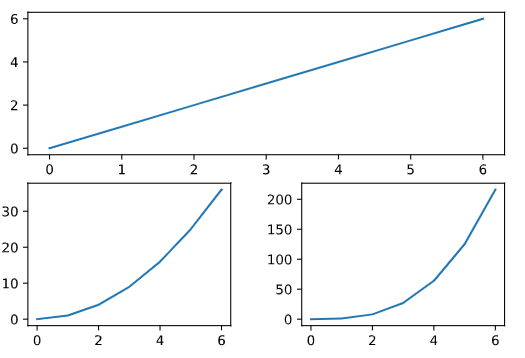
\includegraphics[scale=.55]{subadj}
	\end{minipage} \\
	We can add a \textbf{legend} to our graph, be either passing a list of strings to the .legend( ) method or passing the keywords label=`` " to the .plot method and then calling plt.legend( ) afterwards with no parameters.
	\begin{lstlisting}[language=Python]
	months = range(12)
	hyrule = [63, 65, 68, 70, 72, 72, 73, 74, 71, 70, 68, 64]
	kakariko = [52, 52, 53, 68, 73, 74, 74, 76, 71, 62, 58, 54]
	
	plt.plot(months, hyrule) # could also pass label="Hyrule"
	plt.plot(months, kakariko) # could also pass label="Kakariko"
	
	plt.legend(["Hyrule", "Kakariko"], loc=8) # default loc is 'best position'
	
	plt.show() \end{lstlisting}\vspace*{1mm}
	We can \textbf{modify tick marks} by creating an axes object and modifying the axes of that specific subplot.
	\begin{minipage}[c]{10cm}
	\begin{lstlisting}[language=Python]
	month_names = ["Jan", "Feb", "Mar", "Apr", 
	               "May", "Jun", "Jul", "Aug", 
	               "Sep","Oct", "Nov", "Dec"]
	
	months = range(12)
	conversion = [0.05, 0.08, 0.18, 0.28, 0.4, 0.66, 
	              0.74, 0.78, 0.8, 0.81, 0.85, 0.85]
	
	plt.xlabel("Months")
	plt.ylabel("Conversion")
	
	plt.plot(months, conversion)
	
	ax = plt.subplot() # create axes object
	ax.set_xticks(months) # set x ticks to months
	ax.set_xticklabels(month_names) # string labels
	ax.set_yticks([0.10, 0.25, 0.5, 0.75])
	ax.set_yticklabels(["10%", "25%", "50%", "75%"])
	
	plt.show() \end{lstlisting}\vspace*{1mm}
	\end{minipage}
	\begin{minipage}[c]{7cm}
		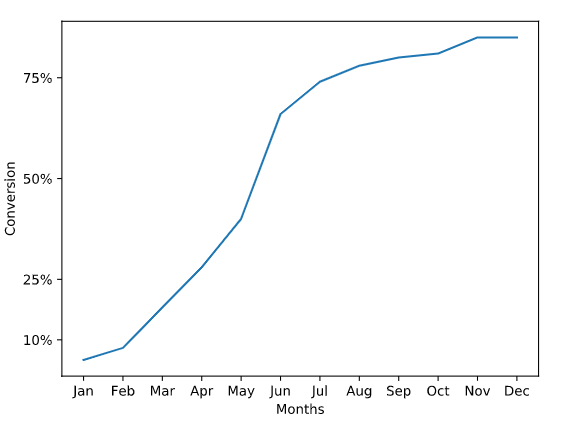
\includegraphics[scale=.52]{ticks}
	\end{minipage} \\
	We can create \textbf{figures} and save them to an output file on our system using the following commands.
	\begin{lstlisting}[language=Python]
	plt.close('all') # clear all existing plots before new one is plotted
	plt.figure(figsize=(7,3)) # creat a figure with width = 7in, height = 3in
	plt.plot(years, power_generated) # plot our data (instead of showing, save to file)
	plt.savefig('power_generated.png') # can also save as .pdf or .svg \end{lstlisting} \newpage
%%%% PAGE 19 %%%%
	\noindent LIME GRAPHING PROJECT
	\begin{lstlisting}[language=Python]
	months = ["Jan", "Feb", "Mar", "Apr", "May", "Jun", "Jul", "Aug", "Sep", "Oct", 
	          "Nov", "Dec"]
	
	visits_per_month = [9695, 7909, 10831, 12942, 12495, 16794, 14161, 12762, 
	                    12777, 12439, 10309, 8724]
	
	# numbers of limes of different species sold each month
	key_limes_per_month = [92.0, 109.0, 124.0, 70.0, 101.0, 79.0, 106.0, 101.0, 
	                       103.0, 90.0, 102.0, 106.0]
	persian_limes_per_month = [67.0, 51.0, 57.0, 54.0, 83.0, 90.0, 52.0, 63.0, 
	                           51.0, 44.0, 64.0, 78.0]
	blood_limes_per_month = [75.0, 75.0, 76.0, 71.0, 74.0, 77.0, 69.0, 80.0, 
	                         63.0, 69.0, 73.0, 82.0]
	
	plt.figure(figsize=(12,8)) # create new figure
	ax1 = plt.subplot(1,2,1) # axes object for left plot
	x_values = range(len(months))
	plt.plot(x_values, visits_per_month, marker='o')
	plt.xlabel("Months")
	plt.ylabel("Number of Visits")
	ax1.set_xticks(x_values)
	ax1.set_xticklabels(months)
	plt.title("Number of Visits per Month")
	
	ax2 = plt.subplot(1,2,2) # axes object for right plot
	plt.plot(x_values, key_limes_per_month, color='green', label='Key Limes')
	plt.plot(x_values, persian_limes_per_month, color='orange', label='Persian Limes')
	plt.plot(x_values, blood_limes_per_month, color='red', label='Blood Limes')
	plt.legend()
	ax2.set_xticks(x_values)
	ax2.set_xticklabels(months)
	plt.title("Lime Sales by Type per Month")
	
	plt.subplots_adjust(wspace=0.3)
	plt.savefig("LimeGraphComparison.png")
	plt.show() \end{lstlisting}\vspace*{1mm}
	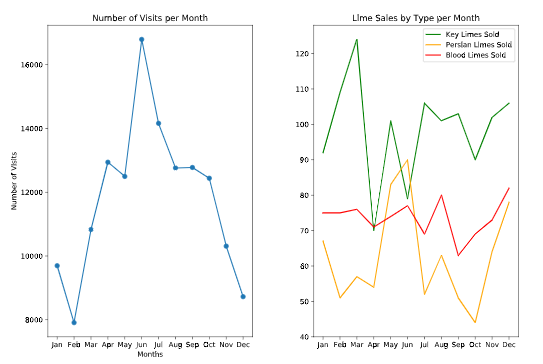
\includegraphics[scale=.95]{lime} \newpage
%%%% PAGE 20 %%%%
	\subsubsection{Different Plot Types \& Error}
	We can create \textbf{simple bar charts} to compare multiple categories of data with the plt.bar( ) function.\\
	\hspace*{3mm} - Note: We want our x to have the same number of elements as y, often we use range(len(y\_value))
	\begin{minipage}[c]{9cm}
	\begin{lstlisting}[language=Python]
	drinks = ["cappuccino", "latte", "chai", 
	"americano", "mocha", "espresso"]
	sales =  [91, 76, 56, 66, 52, 27]
	# create bar graph
	plt.bar(range(len(drinks)), sales) 
	# create axes object
	ax = plt.subplot()
	ax.set_xticks(range(len(drinks)))
	# label each x to corresponding drinks
	ax.set_xticklabels(drinks, rotation=20)	
	plt.show() \end{lstlisting}\vspace*{1mm}
	\end{minipage}
	\begin{minipage}[c]{8cm}
	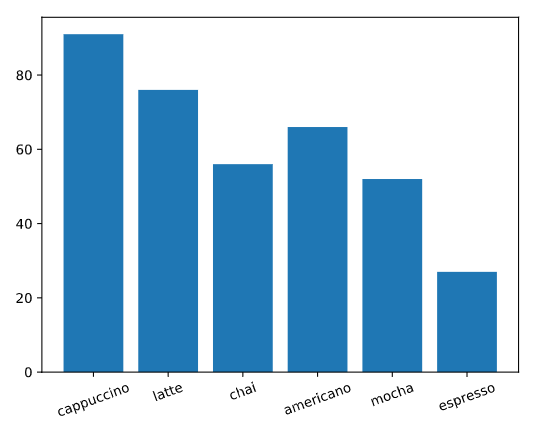
\includegraphics[scale=.5]{barchart}
	\end{minipage} \vspace*{1mm} \\
	We can use \textbf{side-by-side bar charts} to compare two sets of data with the same types of axis values. We must generate the x-axis values using list comprehension (same formula every time). \\
	\begin{minipage}[c]{9.2cm}
	\begin{lstlisting}[language=Python]
	drinks = ["cappuccino", "latte", "chai", 
	          "americano", "mocha", "espresso"]
	sales1 =  [91, 76, 56, 66, 52, 27]
	sales2 = [65, 82, 36, 68, 38, 40]
		
	n = 1  # Current dataset number
	t = 2 # Number of datasets
	d = 6 # Number of sets of bars
	w = 0.8 # Width of each bar
	store1_x = [t*element + w*n for element in 
	            range(d)]
		
	n=2 # 2nd dataset number (use prev. t,d,w)
	store2_x = [t*element + w*n for element in 
	            range(d)]
	
	plt.bar(store1_x, sales1) #plot first bar
	plt.bar(store2_x, sales2) # plot 2nd bar
	plt.show() # display graph \end{lstlisting}\vspace*{1mm}
	\end{minipage}
	\begin{minipage}[c]{8cm}
		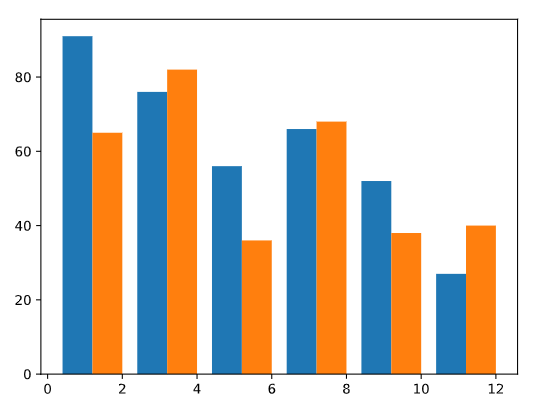
\includegraphics[scale=.57]{sidebyside}
	\end{minipage} \vspace*{1mm} \\
	We can use \textbf{stacked bar charts} to compare two data sets while preserving the total between them. We do this by plotting the first graph, then passing the keyword `bottom=' for the 2nd graph to be on top. \href{https://matplotlib.org/3.1.1/gallery/lines_bars_and_markers/bar_stacked.html}{Click here} for visual of graph style.
	\begin{lstlisting}[language=Python]
	# use datasets from above: drinks, sales1, sales2 
	
	plt.bar(range(len(drinks)), sales1, label='Location 1')
	plt.bar(range(len(drinks)), sales2, bottom=sales1, label='Location 2')
	plt.legend()
	plt.show() \end{lstlisting}\vspace*{1mm}
	We can visually represent uncertainty in our graph through using \textbf{error bars}, by passing the keywords `yerr' and `capsize' to the plt.bar( ) function. Note that you can change the error for each y-value by passing a list to yerr. (Click above link in stacked bar chart section to see example of yerr).
	\begin{lstlisting}[language=Python]
	drinks = ["cappuccino", "latte", "chai", "americano", "mocha", "espresso"]
	ounces_of_milk = [6, 9, 4, 0, 9, 0]
	error = [0.6, 0.9, 0.4, 0, 0.9, 0]
	
	plt.bar(range(len(drinks)), ounces_of_milk, yerr=error, capsize=5)
	plt.show() \end{lstlisting} \newpage
%%%% PAGE 21 %%%%
	\noindent Just like in bar charts, we can represent \textbf{error in line graphs} by using the .fill\_between( ) method and passing x-values, lower y bounds, upper y bounds, and alpha. We also must use list comprehension to calculate the upper/lower y bounds from the original y-values. (note: alpha changes error transparency).\\
	\begin{minipage}[c]{9.2cm}
	\begin{lstlisting}[language=Python]
	months = range(12)
	month_names = ["Jan", "Feb", "Mar", "Apr", 
	               "May", "Jun", "Jul", "Aug", 
	               "Sep", "Oct", "Nov", "Dec"]
	revenue = [16000, 14000, 17500, 19500, 
	           21500, 21500, 22000, 23000, 
	           20000, 19500, 18000, 16500]
	
	y_lower = [0.9*i for i in revenue]
	y_upper = [1.1*i for i in revenue]
	
	ax = plt.subplot()
	plt.fill_between(months, y_lower, y_upper, 
	                 alpha=0.2)
	plt.plot(months, revenue, marker=".")
	ax.set_xticks(months)
	ax.set_xticklabels(month_names)
	plt.show() \end{lstlisting}\vspace*{1mm}
	\end{minipage}
	\begin{minipage}[c]{8cm}
		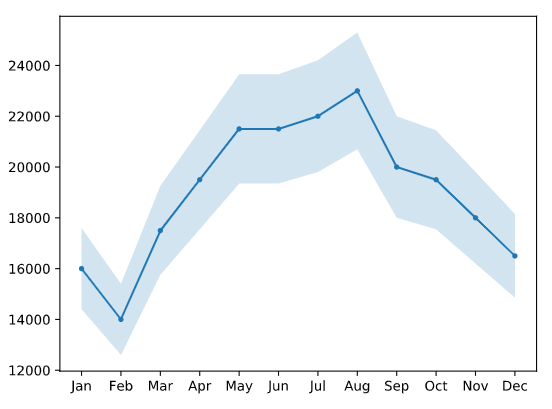
\includegraphics[scale=.57]{lineerr}
	\end{minipage} \vspace*{1mm} \\
	We can use \textbf{pie charts} to display elements of a data set as proportions of a whole by using plt.pie( ). Note that it will be tilted and we don't want this, so we must past plt.axis(``equal'') to flatten. Labeling a pie chart can be done in two different ways: \\ 
	\hspace*{3mm} - Use plt.legend( ) to create a color coded legend for each slice \\
	\hspace*{3mm} - Pass the keyword \textit{labels=` '} to plt.pie( ) to add labels on each slice \\
	We can also add the percent to the pie chart by passing the keyword autopct=` ' to the plt.pie( ) function
	\begin{lstlisting}[language=Python]
	payment_method_names = ["Card Swipe", "Cash", "Apple Pay", "Other"]
	payment_method_freqs = [270, 77, 32, 11]
	
	plt.pie(payment_method_freqs, autopct='%0.1f%%') # percent to 1 decimal place with % sign
	plt.axis('equal') # flatten our pie chart
	plt.legend(payment_method_names) # create color coded legend for graph
	plt.show() \end{lstlisting}\vspace*{1mm}
	We can create \textbf{histograms} to find a more intuitive sense for a dataset and see how many values fall in between a certain range. We do this by calling plt.hist( ). Note that we can also compare two different distribution by plotting multiple histograms, but we need to know a few keywords for this: \\
	\hspace*{3mm} - \textit{bins=} changes the number of bins to divide the data into (default is 10) \\
	\hspace*{3mm} - \textit{range=( )} to change the x-axis display value range \\
	\hspace*{3mm} - \textit{alpha=} to change the transparency of our graphs (lets us see overlap of 2 histograms) \\
	\hspace*{3mm} - \textit{histtype=`step'} will only draw the outline of our graphs (good for viewing overlap) \\
	\hspace*{3mm} - \textit{normed=True} will normalize the data so total shaded area = 1 (good for different sized data sets)
	\begin{minipage}[c]{9cm}
	\begin{lstlisting}[language=Python]
	# plot the first histogram (blue)
	plt.hist(sales_times1, bins=20, alpha=0.4, 
	         normed=True)
	         
	# plot the second histogram (orange)
	plt.hist(sales_times2, bins=20, alpha=0.4, 
	         normed=True)
	         
	plt.show() # overlap is brown \end{lstlisting}\vspace*{1mm}
	\end{minipage}
	\begin{minipage}[c]{9cm}
	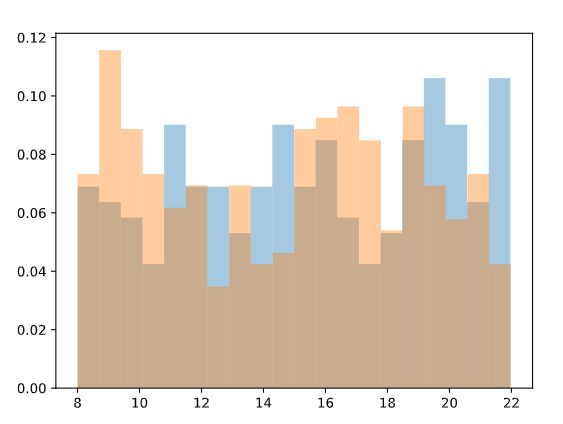
\includegraphics[scale=.48]{multhist}
	\end{minipage} \newpage
%%%% PAGE 22 %%%%
	\subsubsection{Selecting the Correct Visualization}
	The three steps of the data visualization process are \textit{preparing, visualizing, and styling}. We often wonder which chart to use (the visualization stage), so we can use this diagram to help us select a chart based on the data we are using and the question we are focusing on: \\~\\
	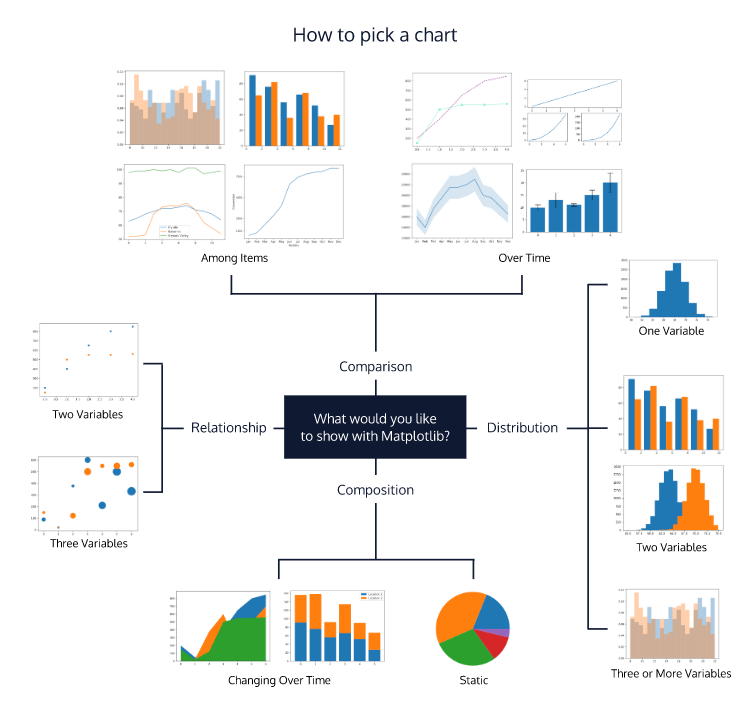
\includegraphics[scale=.8]{visdiag} \\
	\textbf{Composition Charts} - Used when asking ``what are the parts of some whole" or ``what is the data made of". Data pertaining to proportions or percentages as a whole are a good fit. \vspace*{2mm} \\
	\textbf{Distribution Charts} - Data in large quantities work well (see patterns, re-occurrences, clustering). Data that we want to see its ``distribution'' of is a good fit (such as seeing a normal dist. in statistics). \vspace*{2mm} \\
	\textbf{Relationship Charts} - Used when asking ``how do variables relate to each other". Data with two or more variables area good fit (used to see correlation between them). \vspace*{2mm} \\
	\textbf{Comparison Charts} - Used when asking ``how do variables compare to each other". Data must have multiple variables and are being used to compare against one another. \\~\\
	\textbf{Resources}: \\
	1) \href{https://s3.amazonaws.com/codecademy-content/courses/matplotlib/data_vis_matplotlib_cheatsheet_v1_revisons.pdf}{Matplotlib Cheat Sheet} from Codecademy. \\
	2) \href{https://matplotlib.org/tutorials/index.html}{Tutorials from Matplotlib website}. \\
	3) See `Constellation` project in Python folder for \underline{scatter plot} and \underline{3d rotations} in Matplotlib. \newpage
%%%% PAGE 23 %%%%
	\subsection{Introduction to Seaborn}
	Seaborn is a Python data visualization library that provides simple code to create elegant visualizations for statistical exploration and insight. Seaborn is based on Matplotlib, but improves on Matplotlib in several ways: \\	
	\hspace*{3mm} - Seaborn provides a more visually appealing plotting style and concise syntax. \\
	\hspace*{3mm} - Seaborn natively understands Pandas DataFrames, making it easier to plot data directly from CSVs. \\
	\hspace*{3mm} - Seaborn can easily summarize Pandas DataFrames with many rows of data into aggregated charts. \vspace*{2mm}\\
	Assume the following imports are all done in the examples:
	\begin{lstlisting}[language=Python]
	import pandas as pd
	from matplotlib import pyplot as plt
	import seaborn as sns
	import numpy at np \end{lstlisting}\vspace*{1mm}
	Seaborn has a much simpler way to create \textbf{bar charts} compared to Matplotlib, and we can do so with the function sns.barplot( ) and the following three keywords: \\
	\hspace*{3mm} - \textit{data=} is a Pandas DataFrame that contains the data. \\
	\hspace*{3mm} - \textit{x=} is a string that tells Seaborn which column in the DataFrame contains x-labels. \\
	\hspace*{3mm} - \textit{y=} is a string that tells Seaborn which column in the DataFrame contains y-values. \\ 
	Note: By default, Seaborn will aggregate and plot the mean of each category. 
	\begin{lstlisting}[language=Python]
	df = pd.read_csv('results.csv') # contains columns 'Gender' and 'Mean Satisfaction'
	sns.barplot(x='Gender', y='Mean Satisfaction', data= df)
	plt.show()\end{lstlisting}\vspace*{1mm}
	Seaborn can also calculate \textbf{aggregate statistics} (a single number used to describe a set of data) for large datasets. We can use NumPy to calculate these aggregates from our DataFrames. 
	\begin{lstlisting}[language=Python]
	gradebook = pd.read_csv("gradebook.csv")
	
	assignment1 = gradebook[gradebook.assignment_name == 'Assignment 1']
	asn1_median = np.median(assignment1.grade)	
	
	# Seaborn will agregate grade by assignment_name and plot average grade for both 
	# assignment 1 and assignment 2
	sns.barplot(data=gradebook, x='assignment_name', y='grade')
	plt.show()\end{lstlisting}\vspace*{1mm}
	By default, the barplot( ) function will place \textbf{error bars} (the range of values that might be expected for that bar) on all of our bars in the graph. By default, Seaborn uses a \textit{bootstrapped confidence interval} at a 95\% confidence level (but we can change the error types of these bars using the \textit{ci=} keyword). 
	\begin{lstlisting}[language=Python]
	gradebook = pd.read_csv("gradebook.csv")
	
	# change error bars to one standard deviation instead of 95% confidence intervals
	sns.barplot(data=gradebook, x="name", y="grade", ci='sd')\end{lstlisting}\vspace*{1mm}
	We can \textbf{calculate different aggregates} than just the mean of our data (Seaborn's default aggregate) by using the \textit{estimator=} keyword, which accepts any function that works on a list. Some examples: \\
	\hspace*{3mm} - np.median : use if our data has many outliers. \\
	\hspace*{3mm} - len : how many times a value appears (categorical data). 
	\begin{lstlisting}[language=Python]
	df = pd.read_csv("survey.csv")
	
	# Show how many men and women answered the survey (grouped by gender)
	sns.barplot(data=df, x='Gender', y='Response', estimator=len)
	# Show the median response value aggregated by gender
	sns.barplot(data=df, x='Gender', y='Response', estimator=np.median)\end{lstlisting}\newpage
%%%% PAGE 24 %%%%
	\noindent We can \textbf{aggregate by multiple columns} to visualize nested categorical variables. We can compare two columns at once by using the keyword \textit{hue=} to add a nested categorical variable to the plot.
	\begin{minipage}[c]{9cm}
	\begin{lstlisting}[language=Python]
	gradebook = pd.read_csv("gradebook.csv")
	
	# Visualize mean response value by gender 
	# with age range nested
	sns.barplot(data=df, x="Gender", 
	            y="Response", 
	            hue="Age Range")
	plt.show() \end{lstlisting}\vspace*{1mm}
	\end{minipage}
	\begin{minipage}[c]{10cm}
		\hspace*{5mm} 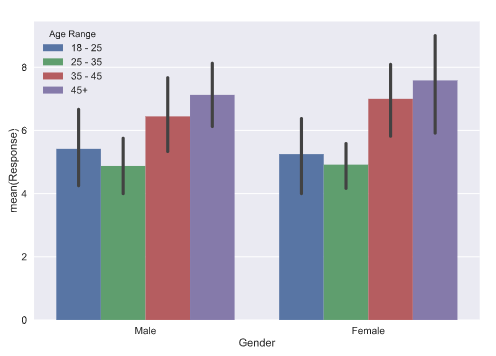
\includegraphics[scale=.5]{seamult}
	\end{minipage} \\
	\subsubsection{Plotting Distributions}
	One of the most powerful aspects of Seaborn is its ability to visualize and compare distributions. Calculating and graphing distributions is integral to analyzing massive amounts of data. We’ll look at how Seaborn allows us to communicate important statistical information through plots. \vspace*{2mm} \\
	We can use \textbf{KDE Plots} (Kernel Density Estimator) to give us the sense of a univariate (only on varaible, `one-dimensional') as a curve. KDE plots are preferable to histograms because they smooth the datasets and allow us to generalize over the shape of our data (and aren't beholden to specific data points).
	\begin{minipage}[c]{10.3cm}
	\begin{lstlisting}[language=Python]
	# Take in the data from the CSVs as NumPy arrays:
	s1 = np.genfromtxt("dataset1.csv", delimiter=",")
	s2 = np.genfromtxt("dataset2.csv", delimiter=",")
	s3 = np.genfromtxt("dataset3.csv", delimiter=",")
	s4 = np.genfromtxt("dataset4.csv", delimiter=",")
	
	sns.set_style("darkgrid") # set style
	
	# Plot the 4 datasets
	sns.kdeplot(s1, shade=True) 
	sns.kdeplot(s2, shade=True) # bimodal (two peaks)
	sns.kdeplot(s3, shade=True) # skewed left
	sns.kdeplot(s4, shade=True) # normal-ish
	plt.legend(['set 1', 'set 2', 'set 3', 'set 4'])
	plt.show() \end{lstlisting}\vspace*{1mm}
	\end{minipage}
	\begin{minipage}[c]{10cm}
	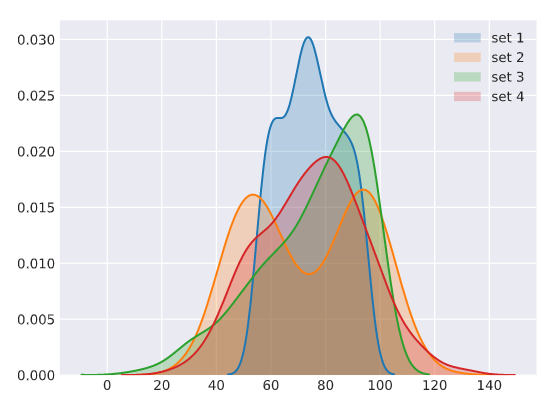
\includegraphics[scale=.48]{kde}
	\end{minipage} \\
	We can use \textbf{box plots} to show us the range of our dataset, give us an idea about where a significant portion of our data lies, and whether or not any outliers are present. We interpret a box plot as: the \textit{box} represents interquartile range, the \textit{line in the middle} of the box is the mean, the \textit{end lines} are the first and third quartiles, and the \textit{diamonds} show outliers. \\
	\hspace*{3mm} - An advantage of box plots over KDE is that it's easy to plot multiples and compare range of values. \\
	\hspace*{3mm} - Note that it shows the range of values and not the curve (distribution) of the datasets. \\
	\begin{minipage}[c]{10.3cm}
	\begin{lstlisting}[language=Python]
	n=500
	df = pd.DataFrame({ # using s1-s4 from above
	"label": ["set_one"] * n + ["set_two"] * n + 
	         ["set_three"] * n + ["set_four"] * n,
	"value": np.concatenate([s1, s2, s3, s4])
	})
	
	sns.set_style("darkgrid") # set style
	
	# Plot the 4 datasets using the dataframe
	sns.boxplot(data=df, x='label', y='value')
	plt.show()	\end{lstlisting}\vspace*{1mm}
	\end{minipage}
	\begin{minipage}[c]{10cm}
	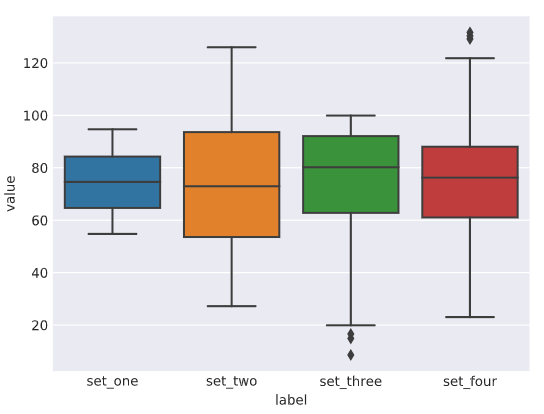
\includegraphics[scale=.48]{bpdist}
	\end{minipage} \newpage
%%%% PAGE 25 %%%%
	\noindent We can use \textbf{violin plots} to compare distributions by giving us an estimation of the dataset. It can show us the distribution (like the KDE plot) and information about the median/interquartile range (like the box plot). They are trickier to read and can be broken down to the following parts: \\
	\hspace*{3mm} - There are two \textit{KDE plots} that are symmetrical along the center line. \\
	\hspace*{3mm} - A \textit{white dot} represents the median. \\
	\hspace*{3mm} - The \textit{thick black line} in the center of each violin represents the interquartile range. \\
	\hspace*{3mm} - The \textit{lines extending from the center} are 95\% confidence intervals for our data. \\
	\begin{minipage}[c]{10.3cm}
	\begin{lstlisting}[language=Python]
	# using s1, s2, s3, and s4 from above
	# and using df from above
	
	sns.set_style("darkgrid") # set style
	
	# plot the 4 distributions using violin plot
	sns.violinplot(data=df, x='label', y='value')
	plt.show()
	# notice we see the same distributions from KDE
	# and same ranges from the boxplot \end{lstlisting}\vspace*{1mm}
	\end{minipage}
	\begin{minipage}[c]{10cm}
		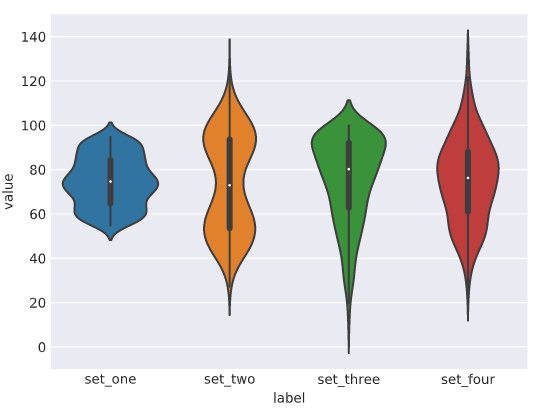
\includegraphics[scale=.48]{violin}
	\end{minipage} \\

	\subsubsection{Styling Graphs}
	Styling your graphs will influence how your audience understands what you're trying to convey. When deciding the style, ask yourself: is it part of a report, is it part of a presentation, is it stand alone with no explanation? These questions will help decide which style to chose in order to best convey your data. \\~\\
	Seaborn has five \textbf{built in themes}: darkgrid, whitegrid, dark, white, and ticks. All of which can be passed into the sns.set\_style( ) method. \vspace*{2mm} \\
	It is important to consider \textbf{background color}. The higher the contrast between you plot color palette and the figure background, the more legible the data visualization will be. \vspace*{2mm} \\
	Including a \textbf{grid} can be helpful when you want your audience to be able to draw their own conclusions about data. Research papers and reports are a good example of when you would want to include a grid.\vspace*{2mm} \\
	We can remove \textbf{spines} from plots (the four black borders that contain the graph) by using sns.despine(), which by default will remove the top/right spines (can pass \textit{left=True, bottom=True} to remove all spines).\vspace*{2mm} \\
	We can \textbf{customize plots for presentation} by using sns.set\_context( ) and passing these keywords: \\
	\hspace*{3mm} - the first parameter adjusts the scale of the plot: `paper', `notebook', `talk', `poster'. \\
	\hspace*{3mm} - \textit{font\_scale=} will change the size of the text. \\
	\hspace*{3mm} - \textit{rc=} will let us change any value in a dictionary (run sns.plotting\_context() to see which values can 
	\hspace*{5.5mm} be changed). \vspace*{2mm} \\
	We can change \textbf{palette color} with two different functions, sns.color\_palette( ) and sns.set\_pallete( ). \\
	\hspace*{3mm} - sns.color\_palette( ) can be saved to a variable, then passed in sns.palplot( ) to see an array of colors. \\
	\hspace*{3mm} - sns.set\_pallete( ) is passed the name of the pallete you want to use for the plot. \vspace*{2mm} \\
	Note: you can also use \href{https://colorbrewer2.org/#type=sequential&scheme=BuGn&n=3}{Color Brewer Palettes} instead of the default Seaborn colors by passing the name and number of colors needed.
	\begin{lstlisting}[language=Python]
	palette = sns.color_palette("bright") # to visualize the colors in a pallete
	sns.palplot(palette) 
	
	sns.set_palette("Paired") # to set the pallete for the plot
	sns.set_palette("Set3", 10) # color brewer pallete with 10 different shades	\end{lstlisting} \vspace*{1mm}
	See `Kiva Loans (Seaborn Project)' in \textit{DS Projects} folder for final Seaborn project.\newpage
%%%% PAGE 26 %%%%
	\subsection{Data Visualization Cumulative Project (Matplotlib)}
	\begin{lstlisting}[language=Python]
	restaurants = pd.read_csv('restaurants.csv')
	orders = pd.read_csv('orders.csv')
	
	##### Q1: What cuisines does FoodWheel offer? What area should they focus on? #####
	
	# count number of different types of cuisines offered (returns int)
	cuisine_options_count = restaurants.cuisine.nunique()
	
	# number of restaurants for each cuisine offered (returns table)
	cuisine_counts = restaurants.groupby('cuisine').name.count().reset_index()
	
	cuisines = cuisine_counts.cuisine.values # list of cuisine names
	counts = cuisine_counts.name.values # number of restaruants of each cuisine
	
	# plot a pie chart of number of restuarants offereing certain cuisines 
	plt.pie(counts, autopct='%d%%', labels=cuisines)
	plt.title('Number of Restaurants Offering Cuisine Types')
	plt.axis('equal')
	plt.show() # see (Figure 1) below
	
	############### Q2: How has average order amount changed over time? ###############
	
	# create new column with month (extract from date column)
	orders['month'] = orders.date.apply(lambda x: x.split('-')[0])
	
	avg_order = orders.groupby('month').price.mean().reset_index() # avg order price
	std_order = orders.groupby('month').price.std().reset_index() # std of order price
	
	bar_heights = avg_order.price.values # average order prices
	bar_errors = std_order.price.values # standard dev of prices
	
	ax = plt.subplot()
	plt.bar(range(len(bar_heights)), bar_heights, yerr=bar_errors, capsize=5)
	plt.ylabel('Average Order Price')
	plt.title('Average Order Price by Month (Figure 2)')
	ax.set_xticks(range(len(avg_order)))
	ax.set_xticklabels(['April', 'May', 'June', 'July', 'August', 'September'])
	plt.show() # see (Figure 2) below
	
	### Q3: How much has each customer on FoodWheel spent over the past six months? ###
	
	c_amount = orders.groupby('customer_id').price.sum().reset_index() # total each cust
	
	plt.hist(c_amount.price.values, range=(0, 200), bins=40)
	plt.xlabel('Total Spent')
	plt.ylabel("Number of Customers")
	plt.title('Customer Expenditure Over 6 Months (Figure 3)')
	plt.show() # see (Figure 3) below	\end{lstlisting}\vspace*{1mm}
	\begin{minipage}[c]{5.5cm}
		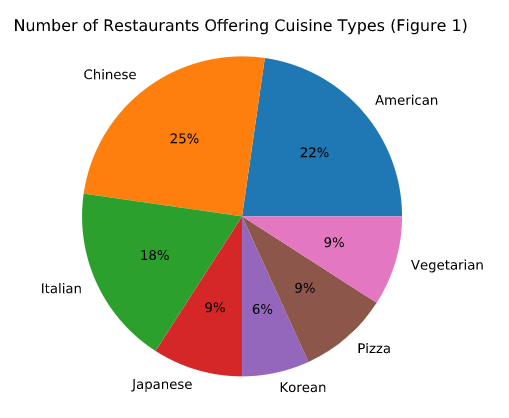
\includegraphics[scale=.39]{figure1}
	\end{minipage}
	\begin{minipage}[c]{6cm}
		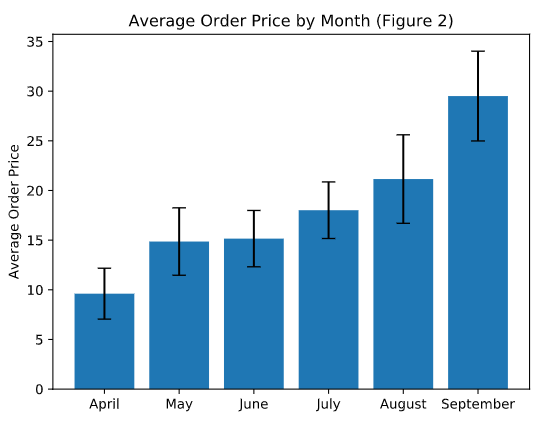
\includegraphics[scale=.39]{figure2}
	\end{minipage}
	\begin{minipage}[c]{6cm}
		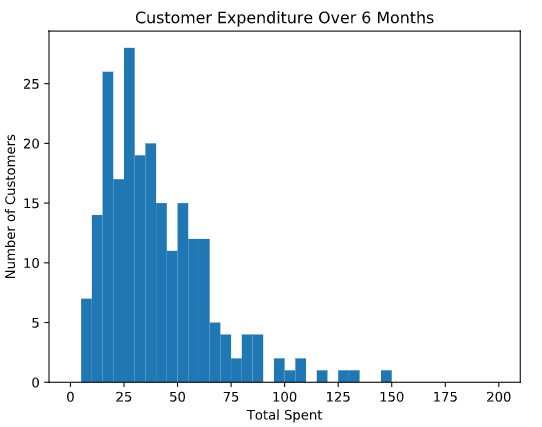
\includegraphics[scale=.39]{figure3}
	\end{minipage} \newpage
%%%% PAGE 27 %%%%
	
	\section{Statistics in Python}
	\subsection{Basic Statistical Calculations}
	We can us the \textbf{NumPy} and \textbf{SciPy} library to find statistical values from CSV's and NumPy arrays. \\
	\hspace*{3mm} - \textbf{mean}: the average value in a list of numbers (sum / number of elements). \\
	\hspace*{3mm} - \textbf{median}: the value that falls in the middle of a sorted dataset (smallest to largest). \\
	\hspace*{8mm} - note: the np.median( ) function will automatically sort the list for you. \\
	\hspace*{3mm} - \textbf{mode}: the most frequently occurring observation in a dataset (can have multiple).\\
	\hspace*{8mm} - note: this will return an object, access mode by var\_name[0][0], frequency by var\_name[1][0]. \\
	\hspace*{8mm} - note 2: if there are two modes, stats.mode( ) will return the smallest value only.
	\begin{lstlisting}[language=Python]
	from scipy import stats
	import numpy as np
	
	greatest_books = pd.read_csv("top-hundred-books.csv")
	author_ages = greatest_books['Ages']
	
	average_age = np.average(author_ages) # mean (42.12)
	median_age = np.median(author_ages) # median (41.0)
	mode_age = stats.mode(author_ages) # mode (38, frequency = 7) \end{lstlisting}\vspace*{1mm}
	\textbf{Variance} ($\sigma^2$) is a descriptive statistic that describes how spread out the points in a data set are. We get this by taking the squared difference of the data points from the mean (X - $\mu$)$^2$, adding them all up, and then finding the average. (note that variance in measured in \textit{units squared}).
	\begin{lstlisting}[language=Python]
	#using the dataframe from above and the author_ages list
	var_age = np.var(author_ages) \end{lstlisting}\vspace*{1mm}
	\textbf{Standard deviation} ($\sigma$) is computed by taking the square root of the variance and is measured in the correct units (easily interpreted and compared to mean). We can expect 68\% of the data to fall within 1 std of the mean, 95\% to fall within 2 std's of the mean, and 99.7\% to fall within 3 std's of the mean.
	\begin{lstlisting}[language=Python]
	#using the dataframe from above and the author_ages list
	var_age = np.std(author_ages) \end{lstlisting}\vspace*{4mm}
	
	\subsection{Histograms}
	A \textbf{histogram} displays the distribution of your underlying data, and reveals interpretable trends. Two keys features of histograms are \textit{bins} and \textit{counts}. \\
	\hspace*{3mm} - bin: a sub-range of value that falls within the range of a dataset (must all be same width). \\
	\hspace*{3mm} - count: the number of values that fall within a bin's range.	\\
	\hspace*{3mm} - np.histogram( ) takes an array, range, and bin count to calculate the frequency for each range. \\
	\hspace*{7mm} - note: the first array returned is the y value, the second is the range up to the following number.
	\begin{lstlisting}[language=Python]
	transactions = pd.read_csv("transactions.csv")
	times = transactions["Transaction Time"].values # create numpy array
	cost = transactions["Cost"].values # create numpy array
	
	# find the range of the times 
	min_time = np.amin(times) # 0.02661518360957871
	max_time = np.amax(times) # 23.675374635328755
	range_time = max_time - min_time # 23.648759451719176
	
	times_hist = np.histogram(times, range=(0,24), bins=4)
	# (array([101, 231, 213, 455]), array([ 0.,  6., 12., 18., 24.])) 
	# example interpetation: range 0-5.9 has 101 values, 6-11.9 has 231 values \end{lstlisting} \newpage
%%%% PAGE 28 %%%%
	\noindent Histograms are typically viewed \textbf{graphically}, and it becomes harder to interpret the np.histogram( ) function as our number of bins increase. By using plt.hist( ) from matplotlib and the same parameters as np.histogram( ) we can create a visual to see and trends in our data. 
	\begin{lstlisting}[language=Python]
	# using times list from above
	plt.hist(times, range=(0,24), bins=4) # this will graphiclly display times_hist above\end{lstlisting}\vspace*{1mm}
	When plotting a histogram, it’s essential to \textbf{select bins that fully capture the trends} in the underlying data. Often, this will require some guessing and checking. By changing the number of bins in our example above from 4 to 24, we can see that instead of the highest frequency being 18-24 (with 4 bins), the highest values are now from 17-22 (with 24 bins). \\~\\
	Now that we can plot and find values of a histogram, we will learn \textbf{how to describe a histogram} to communicate the correct information. We will take a look at five features of a dataset. \\
	\hspace*{3mm} - center: we will use average and median as our measure of centrality. \\
	\hspace*{3mm} - spread: we will us the minimum, maximum, and range as our measure. \\
	\hspace*{3mm} - skew: the symmetry of our data (can be symmetric, right-skew, or left-skew). \\
	\hspace*{3mm} - modality: the number of peaks in a dataset (uniform(0), unimodal(1), bimodal(2), multimodal(2+)). \\
	\hspace*{3mm} - outliers: a point far away from the rest of the data (report and investigate). \vspace*{1mm} \\
	\begin{minipage}[c]{8cm}
		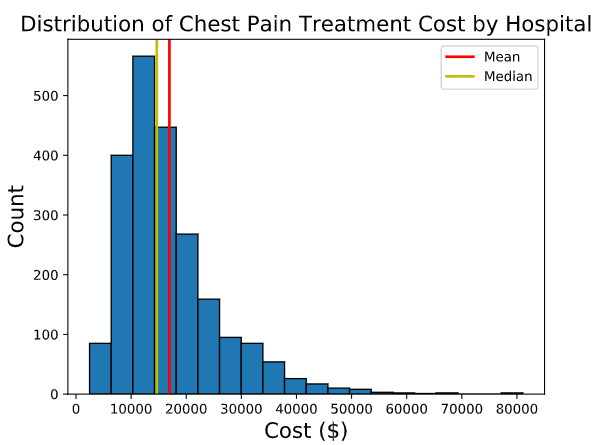
\includegraphics[scale=.5]{chest}
	\end{minipage}
	\begin{minipage}[c]{9.5cm}
	This histogram displays the distribution of chest pain cost for over 2,000 hospitals across the United States. The average and median costs are \textit{\$16,948} and \textit{\$14,659.6}, respectively. Given that the data is \textit{unimodal}, with one local maximum and a \textit{right skew}, the fact that the average is \textit{greater} than the median, matches our expectation. The range of costs is very large, \textit{\$78,623}, with the smallest cost equal to \textit{\$2,459} and the largest cost equal to \textit{\$81,083}. There is one hospital, \textit{Bayonne Hospital Center}, that charges far more than the rest at \textit{\$81,083}.
	\end{minipage} \vspace*{4mm}

	\subsection{Quartiles, Quantiles, and Interquartile Range}
	A common way to communicate a high-level overview of a dataset is to find the values that split the data into four groups of equal size, called \textbf{quartiles} (split into Q1, Q2, Q3, Q4). \\
	\hspace*{3mm} - Q2: this is the middle value (to find it, sort the list and take the median of it). \\
	\hspace*{3mm} - Q1: this is the middle of all the values below Q2 (between minimum and median). \\
	\hspace*{3mm} - Q3: this is the middle of all the value above Q3 (between median and max). \\
	\hspace*{3mm} - note: when calculating Q1 and Q3, you can include or exclude the median from the calculation. \vspace*{2mm} \\
	We can use \textbf{NumPy to find quartiles} by using the \textit{np.quantile( )} function (a quartile is just a specific quantile). We pass two parameters to it, the dataset and a number between 0-1 (quartile percent). 
	\begin{lstlisting}[language=Python]
	from song_data import songs
	import numpy as np
	
	songs_q1 = np.quantile(songs, 0.25) # Q1 (25%)
	songs_q2 = np.quantile(songs, 0.5) # Q2 (50%)
	songs_q3 = np.quantile(songs, 0.75) # Q3 (75%)	\end{lstlisting}\vspace*{1mm}
	Quartiles are so commonly used that the three quartiles, along with the minimum and maximum values of a dataset, are called the \textbf{five-number summary of the dataset}. These help you quickly get a sense of the range, centrality, and spread of the dataset. \newpage
%%%% PAGE 29 %%%%
	\noindent \textbf{Quantiles} are similar to quartiles, but can be expressed as any number (not just split into four). If you have \textit{n} quantiles, it will split the data into \textit{n+1} groups of equal size. Similar to above, we will use NumPy's \textit{np.quantile( )} function to separate the data. To evenly separate the data into multiple quantiles, we pass a list as our parameter. 
	\begin{lstlisting}[language=Python]
	quartiles = np.quantile(songs, [0.25, 0.5, 0.75]) # create quartiles (split into 4)
	deciles = np.quantile(songs, [i/10 for i in range(1,10)]) 
	# list comprehension to find quantile for every 10% (split into 10) \end{lstlisting}\vspace*{1mm}
	Common quantiles: \\
	\hspace*{3mm} - 2-quantile: splits the data in two groups of equal size (also known as the median). \\
	\hspace*{3mm} - 4-quantiles: split the data into four groups of equal size (also known as quartiles). \\
	\hspace*{3mm} - percentiles: split the data into 100 groups (used to compare new data points to dataset). \\~\\
	The \textbf{interquartile range (IQR)} is a descriptive statistic that tries to solve the problem of outliers affecting our range of a dataset. The IQR ignores the tails of the dataset, so you know the range around-which your data is centered. The IQR is the difference between Q3 and Q1 (the middle 50\%). \vspace*{1mm} \\
	We can calculate IQR by hand using NumPy, or find \textbf{IQR in SciPy} by using the \textit{iqr( )} function. Note that IQR is robust, meaning outliers have little impact on it, so two datasets IQR can be identical even with different outliers.
	\begin{lstlisting}[language=Python]
	from scipy.stats import iqr
	
	q1 = np.quantile(songs, 0.25) # calculate Q1
	q3 = np.quantile(songs, 0.75) # calculate Q3
	interquartile_range = q3 - q1 # 99.53959000000003
	
	interquartile_range = iqr(songs) # 99.53959000000003 \end{lstlisting}\vspace*{4mm}
	\textbf{Boxplots} are one of the most common ways to visualize a dataset, they give you a sense of the central tendency and spread of the data. Some of the key features of a boxplot are: \\
	\hspace*{3mm} - median: this is the line within the box (half the data above, half below). \\
	\hspace*{3mm} - interquartile range: these are the edges of the box (data between Q1 and Q3). \\
	\hspace*{3mm} - whiskers: these tell us about the spread of the data (usually 1.5 times the IQR, extend to the \hspace*{24mm} min/max values, or one standard deviation away from the box). \\
	\hspace*{3mm} - outliers: points that fall outside the whiskers (represented with a dot or asterisk). \vspace*{1mm} \\
	We can use \textbf{Matplotlib to make boxplots} by passing it a list (or multiple lists). 
	\begin{lstlisting}[language=Python]
	from music_data import two_thousand, two_thousand_one, two_thousand_two
	import matplotlib.pyplot as plt
	
	# create 3 boxplots on one graph
	plt.boxplot([two_thousand, two_thousand_one, two_thousand_two], 
	            labels = ["2000 Songs", "2001 Songs", "2002 Songs"]) \end{lstlisting}\vspace*{1mm}
	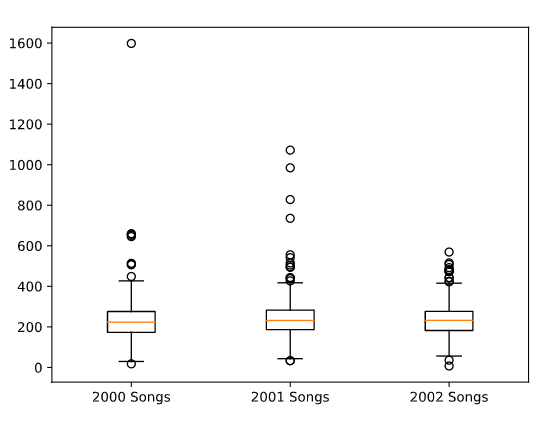
\includegraphics[scale=.4]{bpquart} \newpage
%%%% PAGE 30 %%%%
	\subsection{Introduction to NumPy}
	NumPy includes a powerful data structure known as an \textbf{array}. A NumPy array is a special type of list, and each item can be of any type (strings, numbers, or even other arrays). Note that we can also \textbf{transform a CSV into a NumPy array} using the \textit{np.genfromtxt( )} function. \\
	\hspace*{3mm} - note: the delimiter is how the data is separated in the CSV (could be a tab, colon, comma, etc.).
	\begin{lstlisting}[language=Python]
	import numpy as np
	
	test_1 = np.array([92, 94, 88, 91, 87])
	test_2 = np.genfromtxt('test_2.csv', delimiter=',') \end{lstlisting}\vspace*{1mm}
	Generally, NumPy arrays are more efficient than lists, they allow you to do \textbf{element-wise operations}. These can include addition, subtraction, power, etc on every element in a NumPy array (plus we can add/subtract multiple arrays). 
	\begin{lstlisting}[language=Python]
	test_1 = np.array([92, 94, 88, 91, 87])
	test_2 = np.array([79, 100, 86, 93, 91])
	test_3 = np.array([87, 85, 72, 90, 92])
	test_3_fixed = test_3 + 2 # add 2 to all array elements
	total_grade = test_1 + test_2 + test_3_fixed # add together all 3 arrays
	final_grade = total_grade / 3 # divide each element by 3
	print(final_grade) # [86 93 82 92 90] \end{lstlisting}\vspace*{1mm}
	We can create \textbf{two dimensional arrays} in NumPy (an array of arrays). Note that all arrays must have the same number of elements in order to create a two dimensional array. In statistics, we often use these to represent a set of samples (such as flipping a coin). \\
	\hspace*{3mm} - selecting elements: the syntax is array[row, column]. \\
	\hspace*{3mm} - there are two axes: axis 0 are elements in the same column, axis 1 are elements in the same row.
	\begin{lstlisting}[language=Python]
	student_scores = np.array([[92, 94, 88, 91, 87],
	                           [79, 100, 86, 93, 91],
	                           [87, 85, 72, 90, 92]])
	tanya_test_3 = student_scores [2,0] # 87
	cody_test_scores = student_scores[:,4] # [87 91 92] (all rows, last column) \end{lstlisting}\vspace*{1mm}
	Another useful thing that arrays can do is perform \textbf{element-wise logical operations}, which will return either T/F and can be used to create sub-arrays. 
	\begin{lstlisting}[language=Python]
	porridge = np.array([79, 65, 50, 63, 56, 90, 85, 98, 79, 51])
	
	cold = porridge[porridge < 60] # [50 56 51]
	hot = porridge[porridge > 80] # [90 85 98]
	just_right = porridge[(porridge > 60) & (porridge < 80)] # [79 65 63 79] \end{lstlisting}\vspace*{4mm}
	
	\subsubsection{Statistics with NumPy}
	We can use NumPy's built in function \textit{np.mean( )} to calculate the \textbf{mean} of our arrays (both 1-D and 2-D). We can also use \textbf{logical operators} to find the percent of an array that meets a given condition.
	\begin{lstlisting}[language=Python]
	allergy_trials = np.array([[6, 1, 3, 8, 2], 
	                           [2, 6, 3, 9, 8], 
	                           [5, 2, 6, 9, 9]])
	total_mean = np.mean(allergy_trials) # total of all elements
	trial_mean = np.mean(allergy_trials, axis=1) # for each row
	patient_mean = np.mean(allergy_trials, axis=0) # for each column
	
	print(total_mean) # 5.26666666667
	print(trial_mean) # [ 4.   5.6  6.2]
	print(patient_mean)	# [ 4.33333333  3.     4.     8.66666667  6.33333333] \end{lstlisting} \newpage
%%%% PAGE 31 %%%%

	\noindent \textbf{Outliers} (values that don’t fit within the majority of a dataset) can be used to determine if they were due to an error in sample collection or whether or not they represent a significant but real deviation from the mean. We can use \textit{np.sort( )} to sort our arrays and look at the end points to determine any outliers. \\~\\
	We can calculate the \textbf{median} of our dataset by using the \textit{np.median( )} function. \\~\\
	We can calculate \textbf{percentiles}, where the Nth percentile is defined as the point N\% of samples lie below it. These are useful measurements because they can tell us where a particular value is situated within the greater dataset. To do this, we can use the \textit{np.percentile( )} function. \\
	\hspace*{3mm} - \textit{Five-number summary}: minimum, first quartile, median, third quartile, and maximum. \\
	\hspace*{3mm} - The IQR can be found by subtracting the 25th percentile from the 75th percentile.
	\begin{lstlisting}[language=Python]
	movies_watched = np.array([2, 3, 8, 0, 2, 4, 3, 1, 1, 0, 5, 1, 1, 7, 2])
	
	first_quarter = np.percentile(movies_watched, 25) # pass the array and percentile
	third_quarter = np.percentile(movies_watched, 75) # pass the array and percentile
	interquartile_range = third_quarter - first_quarter # Q3 - Q1
	
	print(first_quarter) # 1.0
	print(third_quarter) # 3.5
	print(interquartile_range) # 2.5 \end{lstlisting}\vspace*{1mm}
	The \textbf{standard deviation} tells us the spread of the data. The larger the standard deviation, the more spread out our data is from the center. The smaller the standard deviation, the more the data is clustered around the mean. We can do this in NumPy with the \textit{np.std( )} function.
	\begin{lstlisting}[language=Python]
	pumpkin = np.array([68, 1820, 1420, 2062, 704, 1156, 1857, 1755, 2092, 1384])
	
	pumpkin_std = np.std(pumpkin)
	print(pumpkin_std) # 611.318378588 \end{lstlisting}\vspace*{4mm}
	
	\subsubsection{Distributions with NumPy}
	We can \textbf{classify} types of distributions in two ways: \vspace*{1mm} \\
	1) Counting the number of \textbf{distinct peaks} present in the graph. Peaks represent concentrations of data. We can describe them as: \textit{Unimodal} (one peak), \textit{Bimodal} (two peaks), \textit{Multimodal} (more than two peaks), or \textit{Uniform} (no distinct peaks, flat). \vspace*{2mm} \\
	2) Describing where most of the numbers are \textbf{relative to the peak}. We can describe them as \textit{Symmetric} (equal amounts of data on both sides of peak), \textit{Skew-Right} (long tail to the right of the peak, most of the data on the left), or \textit{Skew-Left} (long tail on the left of the peak, most of the data is on the right). \vspace*{2mm} \\
	Note: In heavily skewed distributions, the mean becomes a less useful measurement. This means for \textit{symmetric} the mean and median are close together, for \textit{skew-right} this means the mean is greater than the median, and for \textit{skew-left} the mean is less than the median. \\~\\
	\underline{\textbf{Normal Distribution}} \\
	The most common distribution in statistics is known as the \textbf{normal distribution}, which is symmetric and unimodal. Normal distributions are defined by their mean and standard deviation. The mean sets the ``middle" of the distribution, and the standard deviation sets the ``width" of the distribution. \newpage
%%%% PAGE 32 %%%%
	\noindent We can \textbf{generate normally distributed datasets} by using NumPy's function \textit{np.random.normal( )} and passing the following arguments: \\
	\hspace*{3mm} - loc: the mean for the distribution. \\
	\hspace*{3mm} - scale: the standard deviation of the distribution. \\
	\hspace*{3mm} - size: the number of random numbers to generate.
	\begin{lstlisting}[language=Python]
	b_data = np.random.normal(6.7, 0.7, 1000) # mean of 6.7, std of 0.7, 1000 samples \end{lstlisting}\vspace*{1mm}
	We know that the \textbf{standard deviation} affects the ``shape' of our normal distribution. Some rules for the normal distribution are that: 68\% fall within +/- 1 std of the mean, 95\% fall within +/- 2 std's of the mean, and 99.7\% fall within +/- 3 std's of the mean. \\~\\
	\underline{\textbf{Binomial Distribution}} \\
	The \textbf{binomial distribution} can tells us how likely it is for a certain number of ``successes”" to happen, given a probability of success and a number of trials. This distribution is important because it allows us to know how likely a certain outcome is, even when it’s not the expected one. \vspace*{1mm} \\
	Just like before, we can \textbf{generate binomial distribution datasets} by using \textit{np.random.binomial( )} and passing the following arguments: \\
	\hspace*{3mm} - N: the number of samples or trials. \\
	\hspace*{3mm} - P: the probability of success. \\
	\hspace*{3mm} - size: the number of experiments. \\
	Note: we can find the \textbf{probability} of an event occurring by taking the mean with a logical statement. \\
	Note 2: we will get a slightly different number each time since we are using random number generators.
	\begin{lstlisting}[language=Python]
	# we send 500 emails asking for donations with a 5% success rate and we 
	# conducted 10,000 experiments
	emails = np.random.binomial(500, 0.05, size=10000) 
	
	no_emails = np.mean(emails == 0) # probability no one opens the email
	b_test_emails = np.mean(emails >= (500*0.08)) # probability 8% of more open email
	print(no_emails) # 0.0
	print(b_test_emails) # 0.0029 \end{lstlisting}\vspace*{4mm}
	
	\subsection{Hypothesis Testing with SciPy}
	A \textbf{sample} is a subset of the entire population. The mean of each sample is the \textbf{sample mean} and it is an estimate of the \textbf{population mean}. For a population, the mean is a \textit{constant value} no matter how many times it’s recalculated. But with a set of samples, the mean will depend on exactly what samples we happened to choose. From a sample mean, we can then extrapolate the mean of the population as a whole. \vspace*{1mm} \\
	The \textbf{Central Limit Theorem}, states that if we have a large enough sample size, all of our sample means will be sufficiently close to the population mean. \vspace*{1mm} \\
	\textbf{Hypothesis testing} is a mathematical way of determining whether we can be confident that the null hypothesis (usually that the probability of two populations are equal) is false. \\
	\hspace*{3mm} - \textit{Type I error}: occurs when the null hypothesis is rejected even though it is true (``false positive"). \\
	\hspace*{3mm} - \textit{Type II error}: occurs when the null hypothesis is accepted even though it is false (``false negative"). \vspace*{.2mm} \\
	A hypothesis test provides a numerical answer, called a \textbf{p-value}, that helps us decide how confident we can be in the result. In this context, a \textit{p-value} is the probability that we yield the observed statistics under the assumption that the null hypothesis is true. Generally, we want a p-value of less than 0.05, meaning that there is less than a 5\% chance that our results are due to random chance in order to reject the null hypothesis. \newpage
%%%% PAGE 33 %%%%
	\subsubsection{Types of Tests}
	A univariate T-test (\textbf{1 Sample T Test}) compares a sample mean to a hypothetical population mean. We can use the SciPy function \textit{ttest\_1samp( )} and passing it a distribution of values and an expected mean, for which it will return a t-statistic and a p-value. 
	\begin{lstlisting}[language=Python]
	from scipy.stats import ttest_1samp
	
	ages = np.genfromtxt("ages.csv")
	ages_mean = np.mean(ages) # 31
	temp, pval = ttest_1samp(ages, 30)
	print(pval) # 0.5605 \end{lstlisting}\vspace*{1mm}
	A \textbf{2 Sample T-Test} compares two sets of data, which are both approximately normally distributed, and see if there is a significant difference between the two means. We can use the SciPy function \textit{ttest\_ind( )} and passing both distributions as inputs.
	\begin{lstlisting}[language=Python]
	from scipy.stats import ttest_ind
	
	week1 = np.genfromtxt("week1.csv",  delimiter=",")
	week2 = np.genfromtxt("week2.csv",  delimiter=",")
	
	week1_mean = np.mean(week1) # 25.4480593951
	week2_mean = np.mean(week2) # 29.0215681077
	
	temp, pval = ttest_ind(week1, week2)
	print(pval) # 0.000676767690007 \end{lstlisting}\vspace*{1mm}
	Note: The more t-tests we perform to compare data, the more likely we are to get a false positive (Type I error). For example, if we compare n t-tests the probability of making an error is (1-0.95**n). \vspace*{2mm} \\
	When comparing more than two numerical datasets, we use \textbf{ANOVA} (Analysis of Variance) which tests the null hypothesis that all of the datasets have the same mean. If we reject the null hypothesis, we’re saying that at least one of the sets has a different mean; however, it does not tell us which datasets are different. We can use the SciPy function \textit{f\_oneway( )} and pass all the datasets we wish to compare.
	\begin{lstlisting}[language=Python]
	from scipy.stats import f_oneway
		
	a = np.genfromtxt("store_a.csv",  delimiter=",") # mean = 58.3496
	b = np.genfromtxt("store_b.csv",  delimiter=",") # mean - 65.626
	c = np.genfromtxt("store_c.csv",  delimiter=",") # mean = 62.361
	
	temp, pval = f_oneway(a,b,c)
	print(pval) # 0.000153411660078 (reject H0) \end{lstlisting}\vspace*{1mm}
	Assumptions of Numerical Hypothesis Tests: \\
	1. The samples should each be normally distributed (use plt.hist( ) to visualize the distribution). \\
	2. The population standard deviations of the groups should be equal (divide standard deviations and \hspace*{4.5mm} see if ratio is near 1, within 10\% is a good measure).\\
	3. The samples should be independent (info from one dist. shouldn't give info about other dist.). \vspace*{2mm} \\
	After performing an ANOVA test, we can find out which datasets are different with a \textbf{Tukey's Range Test}. We can use the statsmodel function \textit{pairwise\_tukeyhsd( )} by passing a list of all the data, a list of labels, and the significance level (usually 0.05). 
	\begin{lstlisting}[language=Python]
	# using a, b, and c from above example
	from statsmodels.stats.multicomp import pairwise_tukeyhsd
	
	v = np.concatenate([a, b, c]) # list of data
	labels = ['a'] * len(a) + ['b'] * len(b) + ['c'] * len(c) # labels for data
	tukey_results = pairwise_tukeyhsd(v, labels, 0.05)
	print(tukey_results) # prints a chart saying whether to reject or not \end{lstlisting} \newpage
%%%% PAGE 34 %%%%
	\noindent If we have a dataset where the entries are not numbers, but categories instead with two different possibilities for entries, we can use a \textbf{Binomial Test}. A Binomial Test compares a categorical dataset to some expectation. The null hypothesis, in this case, would be that there is no difference between the observed behavior and the expected behavior. We can use the SciPy function \textit{binom\_test( )} by passing the number of successes (x), the total trials (n), and the expected probability of success (p).
	\begin{lstlisting}[language=Python]
	from scipy.stats import binom_test
	
	pval = binom_test(x=510, n=10000, p=0.06)
	print(pval) # 0.000115920327245 (reject H0)
	
	pval2 = binom_test(x=590, n=10000, p=0.06)
	print(pval2) # 0.689152983573 (reject H0) \end{lstlisting}\vspace*{1mm}
	If we have two or more categorical datasets that we want to compare, we should use a \textbf{Chi Square test}. (Useful for problems like: An A/B test where half of users were shown a green submit button and the other half were shown a purple submit button. Was one group more likely to click the submit button?). We can use the SciPy function \textit{chi2\_contingency( )} where there is one input that is a contingency table with: columns = each different condition, rows = different outcomes. In this case, the null hypothesis is that there’s no significant difference between the datasets.
	\begin{lstlisting}[language=Python]
	from scipy.stats import chi2_contingency
	
	# Contingency table
	#         harvester |  leaf cutter
	# ----+------------------+------------
	# 1st gr | 30       |  10
	# 2nd gr | 35       |  5
	# 3rd gr | 28       |  12
	
	X = [[30, 10],
	     [35, 5],
	     [28, 12]]
	chi2, pval, dof, expected = chi2_contingency(X)
	print(pval) # 0.155082308077 (do not reject H0) \end{lstlisting}\vspace*{4mm}
	
	\subsubsection{Sample Size Determination (A/B Tests \& Surveys)}
	An \textbf{A/B Test} is a scientific method of choosing between two options, but in order to determine the sample size necessary we need three numbers for our sample size calculator: \\
	\hspace*{3mm} - \textit{Baseline conversion rate}: number of converted visitors divided by the total number of visitors. \\
	\hspace*{3mm} - \textit{Minimum detectable effect (lift)}: 100 * (target-baseline)/baseline (ex: lift of 50\% means 5\% to 7.5\%)\\
	\hspace*{3mm} - \textit{Statistical significance}: how sure we need to be of the results. \\
	In order to compare the two options, we need a metric. Generally, our metric will be the percent of users who take a certain action after interacting with one of our options. \vspace*{1mm} \\
	Often we do not want to \textit{split an A/B test} as 50/50 in case the new option does not perform well. This will extend the time of our test and lead to more data for the old option, but a Chi-Square test will account for this imbalance. \vspace*{1mm} \\
	Rules: \\
	1) Don’t continue to run a test after the predetermined sample size, until ``significant" results are found. \\
	2) Don’t stop a test before reaching the predetermined sample size, just because your results reach \hspace*{4mm} significance early. \newpage
%%%% PAGE 35 %%%%
	\noindent When we perform a \textbf{survey} we can use a sample size calculator to determine how many people we need to be confident in our results, however we need to know 4 parameters first: \\
	\hspace*{3mm} - \textit{Margin of Error}: the furthest we expect the true value to be from what we measure in the survey. \\
	\hspace*{3mm} - \textit{Confidence level}: the probability that the MOE contains the true proportion (large CI = large SS). \\
	\hspace*{3mm} - \textit{Population size}: 100,000 is default, it depends if it is a global population or within a group.  \\
	\hspace*{3mm} - \textit{Expected Proportion}: a guess of what our result will be (from previous studies, default is 50\%). \\~\\
	Note: whenever we want to make \textbf{comparisons between subpopulations in our survey}, we must use the A/B Test Calculator in order to get our desired survey size. 
	\begin{lstlisting}[language=Python]
	# A/B Testing (finding values and using calculator to find sample size needed)
	import noshmishmosh
	import numpy as np
	
	all_visitors = noshmishmosh.customer_visits
	paying_visitors = noshmishmosh.purchasing_customers 
	total_visitor_count = len(all_visitors)
	paying_visitor_count = len(paying_visitors)
	
	baseline_percent = 100.0 * paying_visitor_count / total_visitor_count
	print(baseline_percent) # 18.6% baseline
	
	payment_history = noshmishmosh.money_spent
	average_payment = np.mean(payment_history)
	new_customers_needed = np.ceil(1240.0/average_payment) # round up
	
	percentage_point_increase = (100.0 * new_customers_needed) / total_visitor_count
	print(percentage_point_increase) # we need a 9.4% increase
	
	minimum_detectable_effect = 100.0 * percentage_point_increase / baseline_percent
	print(minimum_detectable_effect) # 50.54% lift
	
	ab_sample_size = 290 # used calculator to find value \end{lstlisting}\vspace*{4mm}
	
	\section{Data Cleaning / Scraping}
	\subsection{Regular Expressions}
	A \textbf{regular expression (regex)} is a special sequence of characters that describe a pattern of text that should be found, or matched, in a string or document. We can identify how often and where certain pieces of text occur, as well as have the opportunity to replace/update these pieces of text. \vspace*{1mm} \\
	\hspace*{3mm} - \textit{Literals}: our regex contains the exact text we want to match (letters or numbers). \\
	\hspace*{3mm} - \textit{Alternation}: our regex will match the letter/number on either side of the $|$ symbol. \\
	\hspace*{3mm} - \textit{Character sets}: let us match one char from a series of chars within [ ] (good for different spellings). \\
	\hspace*{33mm} ex: con[sc]en[sc]us will match consensus, concensus, consencus, and concencus. \\
	\hspace*{33mm} we can use \^{} to negate certain chars. [\^{}cat] with match any letters but c, a, or t. \\
	\hspace*{3mm} - \textit{Wildcards}: We can use . to match any characters and $\backslash$ to escape a wildcard function. \\
	\hspace*{25mm} ex: we can use ....$\backslash$. to find a 4 letter word with a period, like `lion.' \\
	\hspace*{3mm} - \textit{Ranges}: specify a range of characters to match by using [ - ] (can be multiple ranges also).\\
	\hspace*{3mm} - \textit{Shorthand Character Classes}: represent common ranges (\href{https://www.regular-expressions.info/shorthand.html}{click here for list}). \\
	\hspace*{3mm} - \textit{Grouping}: ( ) allow us to group parts together. ex: It's (4$|$5) pm = It's 4 pm \textit{or} It's 5 pm. \\
	\hspace*{3mm} - \textit{Fixed Quantifiers}: using \{ \} allows us to indicate a quantity/range of characters we want to match. \\
	\hspace*{38mm} ex: $\backslash$w\{3\} (3 word characters), roa\{3,6\}r (roaaar, roaaaar, roaaaaar, roaaaaaar).\newpage
%%%% PAGE 36 %%%%
	\noindent \hspace*{3mm} - \textit{Optional Quantifiers}: we can use ? to indicate a character, or word, is optional. \\
	\hspace*{3mm} - \textit{Kleene star/plus}: * (char appears 0 or more times), + (char appears 1 or more times). \\
	\hspace*{3mm} - \textit{Anchors}: \^{} denotes the beginning of a string, \$ denotes the end of a string (match start/end of text). \\	
	\subsection{Data Cleaning with Pandas}
	Often we have the same data separated into multiple files that all follow the same structure. We can use \textit{glob} with \textit{pandas} in order to \textbf{open and combine multiple files with regex}. 
	\begin{lstlisting}[language=Python]
	import pandas as pd
	import glob
	
	student_files = glob.glob('exams*.csv') # read any csv exams_.csv
	df_list = [] 
	
	for files in student_files: # go through each filename in glob 
		data = pd.read_csv(files) # create a pd dataframe
		df_list.append(data) # append dataframe to our list
	
	students = pd.concat(df_list) # concatenate all dataframes into one \end{lstlisting}\vspace*{1mm}
	In order to \textbf{reshape the data} so that each variable is a separate column and each row is a separate observation, we can us \textit{pd.melt( )} with the following parameters: \\
	\hspace*{3mm} - \textit{frame}: the DataFrame we want to melt. \\
	\hspace*{3mm} - \textit{id\_vars}: the column(s) of the old DataFrame to preserve. \\
	\hspace*{3mm} - \textit{value\_vars}: the column(s) of the old DataFrame that you want to turn into variables. \\
	\hspace*{3mm} - \textit{value\_name}: what to call the column of the new DataFrame that stores the values. \\
	\hspace*{3mm} - \textit{var\_name}: what to call the column of the new DataFrame that stores the variables. \\
	Note: it is also best to us df.columns to rename the columns after melting just to be safe. 
	\begin{lstlisting}[language=Python]
	students = pd.melt(frame=students, id_vars=['full_name', 'gender_age', 'grade'], 
	                   value_vars=['fractions', 'probability'], 
	                   value_name = 'score', var_name = 'exam')	\end{lstlisting}\vspace*{1mm}
	Often we have \textbf{duplicates in our rows}. In order to check, we use \textit{.duplicated( )} which returns a series telling us T/F. Next, we use \textit{.drop\_duplicates( )} to remove the first instance of any duplicates that have all matching column values. Note that if you want to delete every duplicate in a given column, pass the parameter \textit{subset=[`column\_name']}.
	\begin{lstlisting}[language=Python]
	duplicates = students.duplicated() 
	print(duplicates.value_counts()) # 1976 (F), 24 (T)
	students = students.drop_duplicates()
	duplicates = students.duplicated()
	print(duplicates.value_counts()) # 1976 (F), 0 (T)	\end{lstlisting}\vspace*{1mm}
	Often, multiple measurements are recorded in the same column, and we want to separate these out so that we can do individual analysis on each variable. We can \textbf{split by indexing} using the \textit{.str} method.
	\begin{lstlisting}[language=Python]
	# column 'gender_age' has data that looks like 'M16'
	students['gender'] = students.gender_age.str[0:1] # create new column for gender
	students['age'] = students.gender_age.str[1:3] # create new column for age \end{lstlisting}\vspace*{1mm}
	Similar to above, we can also \textbf{split by character} when not all rows in a column are matching lengths.
	\begin{lstlisting}[language=Python]
	# column 'full_name' has data that looks like 'First_name Last_name'
	name_split = students.full_name.str.split(' ') # split column values on space
	students['first_name'] = name_split.str.get(0) # get first name
	students['last_name'] = name_split.str.get(1) # get last name \end{lstlisting} \newpage
%%%% PAGE 37 %%%%
	\noindent We often want to \textbf{look at the types of data} that we are working with. This will help when trying to do any kind of analysis on a given column (such as line graphs) because we will need to convert certain datatypes. We use the \textit{.dtypes} method to find out this information. \vspace*{1.5mm} \\
	We can use regex in Python in combination with Pandas \textit{to\_numeric( )} function to \textbf{transform strings to numerical values} that allow us to perform aggregate statistics on. Along with this, we can also use regex to \textbf{extract numerical data from strings}.
	\begin{lstlisting}[language=Python]
	# score column is '75%' and we want it to be numeric not a string
	students.score = students['score'].replace('[\%]', '', regex=True) # remove all %
	students.score = pd.to_numeric(students.score) # convert to float64	
	
	# grade column is '10th grade' but we only want the numeric value
	students.grade = students['grade'].str.split('(\d+)', expand=True)[1]
	students.grade = pd.to_numeric(students.grade)
	avg_grade = students.grade.mean()
	print(avg_grade) # 10.62 \end{lstlisting}\vspace*{1mm}
	We often have \textbf{data with missing elements} (NaN values). We can use two methods to deal with these: \\
	1) Use \textit{.dropna()} to drop all incomplete rows (pass \textit{subset=[` ']} to remove rows in a certain column). \\
	2) Use \textit{fillna( )} to fill a columns NaN values with a specified new value (can be mean of the column).
	\begin{lstlisting}[language=Python]
	# bill_df is missing num_guests row 3 and bill row 5
	bill_df = bill_df.dropna() # drops the 2 rows with NaN values
	bill_df = bill_df.dropna(subset=['num_guests']) # drop all NaN rows in num_guests
	bill_df = bill_df.fillna(value={"bill":bill_df.bill.mean(), 
	                         "num_guests":bill_df.num_guests.mean()})
	# the above method will fill all NaN values with the mean of the given column \end{lstlisting}\vspace*{1mm}
	
	\subsection{Web Scrapping with Beautiful Soup}
	Beautiful Soup allows us to easily and quickly take information from a website and put it into a DataFrame. This method is used when data is not well-organized in a csv or json file and we have to search for it ourselves. \\~\\
	Rules of Scraping: \\
	1) Always check a website’s Terms and Conditions before scraping (read statement on legal use of data). \\
	2) Do not spam the website with a ton of requests (general rule is one request per second). \\
	3) If the layout of the website changes, you will have to change your scraping code to the new structure. \\~\\
	In order to get the HTML of the website, we need to make a \textbf{request} to get the content of the webpage. From Python's requests library we can use the \textit{.get( )} method to make this request, and the \textit{.content( )} method to store the content of the response.
	\begin{lstlisting}[language=Python]
	import requests
	
	webpage_response = requests.get('https://s3.amazonaws.com/codecademy-content/courses/
	                                 beautifulsoup/shellter.html')
	webpage = webpage_response.content \end{lstlisting}\vspace*{1mm}
	Next, we will want to convert the HTML document to a \textbf{BeautifulSoup object} so we can easily pull the parts we are interested in. We can do this by importing bs4, then passing the webpage.contents and a \textit{parser} to the \textit{BeautifulSoup( )} function.
	\begin{lstlisting}[language=Python]
	from bs4 import BeautifulSoup
	# use webpage variable from above
	soup = BeautifulSoup(webpage, 'html.parser') \end{lstlisting} \newpage
%%%% PAGE 38 %%%%

	\noindent We can navigate through a BeautifulSoup object by calling the \textbf{tag names} on them. These are the characters within the $< >$. We can get the children of a tag by using the \textit{.children} method, and the parent tags by using the \textit{.parent} method.
	\begin{lstlisting}[language=Python]
	# use BeautifulSoup object from above
	for child in soup.div.children:
		print(child) # print child tag of first <div> \end{lstlisting}\vspace*{1mm} 
	If we want to find all of the occurrences of a tag, instead of just the first one, we can use the \textit{.find\_all( )} method, which takes any of the following parameters: \\
	\hspace*{3mm} - \textit{Tags}: can pass any tag as a string (ex: ``h1"). \\
	\hspace*{3mm} - \textit{Regex}: using re.compile(`[ ]') we can pass a regex to the find\_all method. \\
	\hspace*{3mm} - \textit{Lists}: a list of tag names we want to extract. \\
	\hspace*{3mm} - \textit{Attributes}: We can match elements with attributes using .attr=\{ \}. \\
	\hspace*{3mm} - \textit{Functions}: We can create logic functions to get complicated selections.
	\begin{lstlisting}[language=Python]
	soup.find_all("h1") # all <h1> tags
	soup.find_all(re.compile("[ou]l")) # all <ol> and <ul> tags
	soup.find_all(['h1', 'a', 'p']) # all <h1>, <a>, and <p> tags
	soup.find_all(attrs={'class':'banner'}) # all elements in the "banner" class
	
	def has_banner_class_and_hello_world(tag):
		return tag.attr('class') == "banner" and tag.string == "Hello world"
	
	soup.find_all(has_banner_class_and_hello_world) 
	# <div class="banner">Hello world</div>	\end{lstlisting}\vspace*{1mm}
	We can also use \textbf{CSS selectors} and the \textit{.select( )} method to capture the desired elements. We can also use the \textit{.get\_text( )} to retrieve the text inside the tag we call it on. We can use the parameter `$|$' to separate text with different tags within the outside tag. 
	\begin{lstlisting}[language=Python]
	webpage_response = requests.get('https://s3.amazonaws.com/codecademy-content/courses/
	                                 beautifulsoup/cacao/index.html')
	soup = BeautifulSoup(webpage_response.content, 'html.parser') # creat Soup object
	
	rating_tags = soup.find_all(attrs={'class': 'Rating'}) # get all tags
	ratings = [ ]
	for rating in rating_tags[1:]: # skip first element (class header)
		rate_value = rating.get_text() # get text from tag
		ratings.append(float(rate_value)) # convert to float
	
	company_name_tags = soup.select('.Company') # get all tags
	company_names = [ ]
	for company in company_name_tags[1:]: # skip first element (class header)
		c_value = company.get_text() # get text within tag
		company_names.append(c_value)
	
	# create a DataFrame and find 10 highest rated companies (on average)
	df = pd.DataFrame({'Company': company_names, 'Ratings': ratings})
	top_10 = df.groupby('Company').Ratings.mean().nlargest(10)
	
	cocoa_percents = []
	cocoa_percent_tags = soup.select(".CocoaPercent") # get all tags
	for td in cocoa_percent_tags[1:]: # skip first element (class header)
		percent = float(td.get_text().strip('%')) # get percent amount (take off %)
		cocoa_percents.append(percent)
	
	df['CocoaPercentage'] = cocoa_percents # create new column \end{lstlisting} \newpage
%%%% PAGE 39 %%%%

	\section{Machine Learning (Supervised Learning)}
	\subsection{Introduction to Machine Learning}
	\textbf{Supervised Learning} is where the data is labeled and the program learns to predict the output from the input data. SL problems can be further grouped into regression and classification problems: \vspace*{1mm} \\ 
	\hspace*{2mm} 1) \textit{Regression} - we are trying to predict a continuous-valued output. \\
	\hspace*{2mm} 2) \textit{Classification} - we are trying to predict a discrete number of values. \vspace*{2mm} \\ 
	\textbf{Unsupervised Learning} is a type of machine learning where the program learns the inherent structure of the data based on unlabeled examples. \textit{Clustering} is a common unsupervised machine learning approach that finds patterns and structures in unlabeled data by grouping them into clusters. \vspace*{1mm}
	\subsection{Linear Regression}
	When we are trying to find a line that fits a set of data best, we are performing \textbf{Linear Regression}. A line is a rough approximation, but it allows us the ability to explain and predict variables that have a linear relationship with each other. \vspace*{2mm} \\	
	A line is determined by its slope and its intercept (in the form of \textbf{y = mx + b}). When we perform Linear Regression, the goal is to get the ``best" \textit{m} and \textit{b} for our data. \vspace*{2mm} \\
	When we think about how we can assign a slope and intercept to fit a set of points, we have to define what the best fit is. For each data point, we calculate \textbf{loss}, a number that measures how bad the model’s prediction was (also referred to as error). We can think about loss as the \textit{squared distance} from the point to the line. We do the squared distance so that points above and below the line both contribute to total loss in the same way. \vspace*{2mm} \\
	The goal of a linear regression model is to find the slope and intercept pair that \textit{minimizes loss on average across all of the data}.
	\begin{lstlisting}[language=Python]
	x = [1, 2, 3]
	y = [5, 1, 3] # actual y value
	
	#y = 0.5x + 1
	m2 = 0.5
	b2 = 1
	y_predicted2 = [(m2*x + b2) for x in x] # predicted y value
	
	total_loss2 = 0
	for i in range(len(y)):
		total_loss2 += (y[i] - y_predicted2[i])**2 # squared distance
	print(total_loss2) # 13 (total squared distance) \end{lstlisting}\vspace*{1mm}
	We use a process called \textbf{gradient descent} where as we try to minimize loss, we take each parameter we are changing, and move it as long as we are decreasing loss. It’s like we are moving down a hill, and stop once we reach the bottom. The equation to find the gradient of loss as intercept changes (\textbf{b gradient}): $$ \frac{2}{N} \sum_{i=1}^{N} -(y_i - (mx_i + b)) $$ \textit{N} = number of points we have in our dataset. \\ \textit{m} = current gradient guess. \\ \textit{b} = current intercept guess. \newpage
%%%% PAGE 40 %%%%
	\begin{lstlisting}[language=Python]
	# Python function that calculates the gradient loss for intercept (equation above)
	def get_gradient_at_b(x, y, m, b):
		N = len(x) 
		diff = sum([(y-(m*x+b)) for y, x in zip(y, x)])
		b_gradient = (-2 / N) * diff
		return b_gradient \end{lstlisting}\vspace*{1mm}
	Next we can find the way the loss changes as the slope of our line changes (\textbf{m gradient}). We can use this formula: $$ \frac{2}{N} \sum_{i=1}^{N} -x_i(y_i - (mx_i + b)) $$ Once we have a way to calculate both the m gradient and the b gradient, we’ll be able to follow both of those gradients downwards to the point of lowest loss for both the m value and the b value. Then, we’ll have the best m and the best b to fit our data.
	\begin{lstlisting}[language=Python]
	# Python function that calculates the gradient loss for slope (equation above)
	def get_gradient_at_b(x, y, m, b):
		N = len(x) 
		diff = sum([x*(y-(m*x+b)) for y, x in zip(y, x)])
		m_gradient = (-2 / N) * diff
		return m_gradient \end{lstlisting}\vspace*{1mm}
	Now that we know how to calculate the gradient, we want to take a “step” in that direction. However, it’s important to think about whether that step is too big or too small. We can scale the size of the step by multiplying the gradient by a \textbf{learning rate} (the size of the step to take).  
	\begin{lstlisting}[language=Python]
	def step_gradient(x, y, b_current, m_current, learning_rate):
		b_gradient = get_gradient_at_b(x, y, b_current, m_current) 
		m_gradient = get_gradient_at_m(x, y, b_current, m_current)
		b = b_current - (learning_rate * b_gradient) # 'b' step scaled by learning rate
		m = m_current - (learning_rate * m_gradient) # 'm' step scaled by learning rate
		return (b, m) \end{lstlisting}\vspace*{1mm}
	How do we know when we should stop changing the parameters m and b? How will we know when our program has learned enough? \textbf{Convergence} is when the loss stops changing (or changes very slowly) when parameters are changed. \vspace*{2mm} \\
	We want our program to be able to iteratively learn what the best m and b values are. So for each m and b pair that we guess, we want to move them in the direction of the gradients we’ve calculated. We have to choose a \textbf{learning rate}, which will determine how far down the loss curve we go. A \textit{small learning rate} will take a long time to converge (might run out of time or cycles before getting an answer) while a \textit{large} learning rate might skip over the best value (might never converge). \vspace*{1mm} \\
	Finding the absolute best learning rate is not necessary for training a model. You just have to find a learning rate large enough that gradient descent converges with the efficiency you need, and not so large that convergence never happens. \vspace*{1mm}
	\begin{lstlisting}[language=Python]
	def gradient_descent(x, y, learning_rate, num_iterations):
		b = 0
		m = 0
		for step in range(num_iterations):
			b, m = step_gradient(b, m, x, y, learning_rate)
		return (b,m) 
	
	months = [1, 2, 3, 4, 5, 6, 7, 8, 9, 10, 11, 12]
	revenue = [52, 74, 79, 95, 115, 110, 129, 126, 147, 146, 156, 184]
	b, m = gradient_descent(months, revenue, 0.01, 1000)
	y = [m*x + b for x in months] # y values for line \end{lstlisting} \newpage
%%%% PAGE 41 %%%%
	\noindent Luckily, we don’t have to build a regression algorithm from scratch every time we want to use linear regression. We can use Python’s scikit-learn library. Scikit-learn, or \textbf{sklearn}, is used specifically for Machine Learning. Inside the linear\_model module, there is a LinearRegression() function we can use. \vspace*{1mm} \\
	You can first create a LinearRegression model, and then fit it to your x and y data. The .fit() method gives the model two variables that are useful to us: \vspace*{.5mm} \\	
	\hspace*{2mm} 1) line\_fitter.coef\_ which contains the slope. \\
	\hspace*{2mm} 2) line\_fitter.intercept\_ which contains the intercept. \vspace*{1.5mm} \\
	We can also use the .predict() function to pass in x-values and receive the y-values that this line would predict. Note that the \textit{number of iterations} and \textit{learning rate} have default values within scikit-learn so we do not need to set them.
	\begin{lstlisting}[language=Python]
	from sklearn.linear_model import LinearRegression
	import matplotlib.pyplot as plt
	import numpy as np
	
	temperature = np.array(range(60, 100, 2))
	temperature = temperature.reshape(-1, 1)
	sales = [65, 58, 46, 45, 44, 42, 40, 40, 36, 38, 38, 28, 30, 
	         22, 27, 25, 25, 20, 15, 5]
	
	line_fitter = LinearRegression() # create liner regression model
	line_fitter.fit(temperature, sales) # fit our data (x,y)
	sales_predict = line_fitter.predict(temperature) # list of predicted y values
	
	plt.plot(temperature, sales, 'o') # plot points
	plt.plot(temperature, sales_predict) # plot predicted line
	plt.show() \end{lstlisting}\vspace*{1mm}
	Linear Regression Project 
	\begin{lstlisting}[language=Python]
	import pandas as pd
	import matplotlib.pyplot as plt
	import numpy as np
	from sklearn import linear_model
	
	df = pd.read_csv("https://s3.amazonaws.com/codecademy-content/programs/data-science-
	                  path/linear_regression/honeyproduction.csv")
	
	# group by year and get total production for year
	prod_per_year = df.groupby('year').totalprod.sum().reset_index()
	X = prod_per_year['year'] # year column
	X = X.values.reshape(-1, 1) # reshape for scikit-learn (1 value per row)
	y = prod_per_year['totalprod'] # totalprod column
	
	regr = linear_model.LinearRegression() # create Linear Regression model
	regr.fit(X, y)
	print(regr.coef_[0]) # slope is first and only item in list (-4951114.285)
	print(regr.intercept_) # 10100974009.52381
	y_predict = regr.predict(X)
	
	# predict the amount of honey produced in 2050
	X_future = np.array(range(2013, 2051)) # array with years 2013-2050
	X_future = X_future.reshape(-1, 1) # reshape for scikit-learn (1 value per row)
	future_predicts = regr.predict(X_future) # predict y values \end{lstlisting} \newpage
%%%% PAGE 42 %%%%
	\subsection{Multiple Linear Regression}
	\textbf{Multiple Linear Regression} uses two or more independent variables to predict the values of the dependent variable. When we have two independent variables, we can create a linear regression plane. It is based on the following equation: $$ y = b + m_1x_1 + m_2x_2 + ... + m_nx_n$$ 
	As with most machine learning algorithms, we have to split our dataset into two datasets: \\
	\hspace*{2mm} 1) \textbf{Training set} - the data used to fit the model. \\
	\hspace*{2mm} 2) \textbf{Test set} - the data partitioned away at the very start of the experiment (to provide an unbiased \hspace*{27mm} evaluation of the model). \vspace*{1mm} \\
	In general, putting 80\% of your data in the training set and 20\% of your data in the test set is a good place to start. We can use \textit{train\_test\_split( )} from sklearn.model\_selection in Python to split our x/y data into these separate sets. We pass in the proportion of the dataset we want for train split and test split (between 0.0 and 1.0). 
	\begin{lstlisting}[language=Python]
	from sklearn.model_selection import train_test_split
	
	streeteasy = pd.read_csv("https://raw.githubusercontent.com/sonnynomnom/Codecademy-
	                          Machine-Learning-Fundamentals/master/StreetEasy/manhattan.
	                          csv")
	
	df = pd.DataFrame(streeteasy)
	# pick our x (independent variable) columns
	x = df[['bedrooms', 'bathrooms', 'size_sqft', 'min_to_subway', 'floor', 
	        'building_age_yrs', 'no_fee', 'has_roofdeck', 'has_washer_dryer', 
	        'has_doorman', 'has_elevator', 'has_dishwasher', 'has_patio', 'has_gym']]
	y = df[['rent']] # our y (dependent variable) columns
	
	# split the test/train data (random state is the seed for random num generator)
	x_train, x_test, y_train, y_test = train_test_split(x, y, train_size = 0.8, 
	                                                  test_size = 0.2, random_state = 6)
	
	print(x_train.shape) # (2831 row, 14 col)
	print(x_test.shape) # (708 row, 14 col)
	print(y_train.shape) # (2831 row, 1 col)
	print(y_test.shape) # (708 row, 1 col)	\end{lstlisting}\vspace*{1mm}
	We use the \textbf{sklearn} LinearRegression( ) function (same as the single linear regression) for the multiple linear regression model. We fit our training set to the model and use that to predict y values for a given plane. 
	\begin{lstlisting}[language=Python]
	# using data from above
	mlr = LinearRegression()
	mlr.fit(x_train, y_train)
	y_predict = mlr.predict(x_test) # predict y values from x_test
	
	# test our model on an apartment in brooklyn
	sonny_apartment = [[1, 1, 620, 16, 1, 98, 1, 0, 1, 0, 0, 1, 1, 0]]
	# note this must be nested list since predict takes one parameter
	
	predict = mlr.predict(sonny_apartment) # use above model to predict
	
	print("Predicted rent: $%.2f" % predict)
	# They are paying $2000 a month, our model predicts $2393.58 (underpaying)	\end{lstlisting} \newpage
%%%% PAGE 43 %%%%
	\noindent Now that we have implemented Multiple Linear Regression, we will learn how to \textbf{tune and evaluate the model}. From the equation at the beginning of the section, the \textit{m} values refer to the coefficients and \textit{b} refers to the intercept. We can print the coefficients by using \textit{.coef\_} and see which coefficients carry the most weight (have the greatest impact on our model).
	\begin{lstlisting}[language=Python]
	# using the data from above
	print(mlr.coef_)
	# [[-302.73009383 1199.3859951     4.79976742  -24.28993151   24.19824177
	#   -7.58272473 -140.90664773   48.85017415  191.4257324  -151.11453388
	#   89.408889    -57.89714551  -19.31948556  -38.92369828]]	\end{lstlisting}\vspace*{1mm}
	In regression, the independent variables will either have a \textbf{positive linear relationship} to the dependent variable, a \textbf{negative linear relationship}, or \textbf{no relationship}. A negative linear relationship means that as X values increase, Y values will decrease. Similarly, a positive linear relationship means that as X values increase, Y values will also increase. One way to find \textbf{correlation} is by graphing a single independent varaible against the dependent variable to visualize the linear relationship between the two. \\~\\
	When trying to evaluate the accuracy of our multiple linear regression model, one technique we can use is \textbf{Residual Analysis}. he difference between the actual value y, and the predicted value $\hat{y}$ is the residual e, where \textbf{e = y - $\mathbf{\hat{y}}$}. \vspace*{1.5mm} \\
	Sklearn comes with a \textit{.score( )} method that returns the coefficient of determination R$^2$ of the prediction. \textbf{R$^2$} is the percentage variation in y explained by all the x variables together. The TSS tells you how much variation there is in the y variable. R$^2$ is defined as 1 - $\frac{u}{v}$ where... \vspace*{1mm} \\
	\hspace*{2mm} - \textit{u} is the residual sum of squares (RSS) calculated by ((y - y\_predict) ** 2).sum() \\
	\hspace*{2mm} - \textit{v} is the total sum of squares (TSS) calculated by ((y - y.mean()) ** 2).sum() \vspace*{2mm} \\
	For example, say we are trying to predict rent based on the size\_sqft and the bedrooms in the apartment and the R$^2$ for our model is 0.72, which means that all the x variables (square feet and number of bedrooms) together explain 72\% variation in y (rent). \vspace*{1mm} \\	
	Now let’s say we add another x variable, building’s age, to our model. By adding this third relevant x variable, the R$^2$ is expected to go up. Let say the new R$^2$ is 0.95. This means that square feet, number of bedrooms and age of the building together explain 95\% of the variation in the rent. \vspace*{1mm} \\	
	The best possible R$^2$ is 1.00 (and it can be negative because the model can be arbitrarily worse). Usually, a R$^2$ of 0.70 is considered good.
	\begin{lstlisting}[language=Python]
	# using the data from above
	print(mlr.score(x_train, y_train)) # R^2 = 0.7725460559817883
	print(mlr.score(x_test, y_test)) # R^2 = 0.8050371975357647 \end{lstlisting}\vspace*{1mm}
	We can then remove independent variables that have low correlations to see if we can improve our $R^2$.
	\begin{lstlisting}[language=Python]
	# using the data from above
	x = df[['bedrooms', 'bathrooms', 'size_sqft', 'floor', 'building_age_yrs']]
	
	print(mlr.score(x_train, y_train)) # 0.7698948202598073
	print(mlr.score(x_test, y_test)) # 0.8089360081246582 \end{lstlisting}\vspace*{1mm}
	As we can see, we removed 9 of the independent variables and still had about the same $R^2$ value. These variables had low correlation and less of an impact on our model compared to the remaining 5. Although $R^2$ did not go up (stayed about the same) our model is now more simple and requires less input. \\~\\
	(See \textit{Yelp Regression} in projects folder for final regression project). \newpage
%%%% PAGE 44 %%%%
	\subsection{Classification: K-Nearest Neighbors}
	Classification is used to predict a discrete label. \textbf{Binary classification} is when the outputs fall under a finite set of possible outcomes, with many situations having only two possible outcomes. \textbf{Multi-label classification} is when there are multiple possible outcomes. To perform these classifications, we use models like \textit{Naive Bayes}, \textit{K-Nearest Neighbors}, and \textit{SVMs}.
	\subsubsection{Distance Formulas}
	\textbf{Euclidean Distance} is the most commonly used distance formula. To find the Euclidean distance between two points, we first calculate the squared distance between each dimension, add them together, and take the square root. The equation is: $$ \sqrt{(a_1-b_1)^2 + (a_2-b_2)^2 + ... + (a_n-b_n)^2} $$
	\begin{lstlisting}[language=Python]
	def euclidean_distance(pt1, pt2): # calculate distance between two lists
		distance = 0
		if len(pt1) != len(pt2):
			return 'Points are not same dimensions'
		distance = sum([(a-b)**2 for a, b in zip (pt1, pt2)]) ** 0.5
		return distance	\end{lstlisting}\vspace*{2mm}
	\textbf{Manhattan Distance} is extremely similar to Euclidean distance. Rather than summing the squared difference between each dimension, we instead sum the absolute value of the difference between each dimension. Computing Manhattan distance is like asking how many blocks away you are from a point. $$ |a_1-b_1| + |a_2-b_2| + ... + |a_n-b_n| $$ Note that Manhattan distance will always be greater than or equal to Euclidean distance.
	\begin{lstlisting}[language=Python]
	def manhattan_distance(pt1, pt2): # calculate distance between two lists
		distance = 0
		if len(pt1) != len(pt2):
			return 'Points are not same dimensions'
		distance = sum([abs(a-b) for a, b in zip(pt1, pt2)])
		return distance\end{lstlisting}\vspace*{2mm}
	\textbf{Hamming distance} only cares about whether the dimensions are exactly equal. When finding the Hamming distance between two points, add one for every dimension that has different values. This is often used in spell checking algorithms. 
	\begin{lstlisting}[language=Python]
	def hamming_distance(pt1, pt2): # calculate distance between two lists
		distance = 0
		for point in range(len(pt1)):
			if pt1[point] != pt2[point]:
				distance += 1
		return distance\end{lstlisting}\vspace*{2mm}
	Now that we have written these functions, we can use the \textbf{SciPy} library functions to calculate these distances. Note that the Hamming distance returns a value between 0 and 1 (this is because it divides by the total number of dimensions).
	\begin{lstlisting}[language=Python]
	from scipy.spatial import distance # import library
	distance.euclidean([1,2], [4,0]) # Euclidean Distance
	distance.cityblock([1,2], [4,0]) # Manhattan Distance
	distance.hamming([5, 4, 9], [1, 7, 9]) # Hamming Distance \end{lstlisting} \newpage
%%%% PAGE 45 %%%%
	\subsubsection{Normalization \& Dataset Splits}
	Many machine learning algorithms attempt to find trends in the data by comparing features of data points. However, there is an issue when the features are on drastically different scales. The goal of \textbf{normalization} is to make every datapoint have the same scale so each feature is equally important. \vspace*{1.5mm} \\ 
	\textbf{Min-max normalization} is one of the most common ways to normalize data. For every feature, the minimum value of that feature gets transformed into a 0, the maximum value gets transformed into a 1, and every other value gets transformed into a decimal between 0 and 1. However, it does not handle outliers very well. The formula is: $$ \frac{value - min}{max - min} $$ \\
	\textbf{Z-score normalization} is a strategy of normalizing data that avoids the outlier issue of min-max. $$ \frac{value - \mu}{\sigma} $$ Here, $\mu$ is the mean value of the feature and $\sigma$ is the standard deviation of the feature. If a value is exactly equal to the mean of all the values of the feature, it will be normalized to 0. If it is below the mean, it will be a negative number, and if it is above the mean it will be a positive number. The size of those negative and positive numbers is determined by the standard deviation of the original feature. If the unnormalized data had a large standard deviation, the normalized values will be closer to 0. \vspace*{1.5mm} \\
	Summary: \\
	\hspace*{2mm} - \textbf{Min-max}: Guarantees all features will have the exact same scale but does not handle outliers well. \\
	\hspace*{2mm} - \textbf{Z-score}: Handles outliers, but does not produce normalized data with the exact same scale. \\~\\
	In order to test the effectiveness of your algorithm, we’ll \textit{split this data} into 3 different sets. \vspace*{1.5mm} \\
	The \textbf{training set} is the data that the algorithm will learn from. Learning looks different depending on which algorithm you are using. In K-Nearest Neighbors, the points in the training set are the points that could be the neighbors. \vspace*{1.5mm} \\
	The \textbf{validation set} is used to compute the accuracy/error of the classifier. The key here is that we know the true labels of every point in the validation set, but we temporarily pretend like we don’t. We can use every point in the validation set as input to our classifier. We then receive a classification for that point, from which we peek at the true label of the validation point to see whether we got it right or not. We can do this for every point in the validation set to compute the \textbf{validation error} (we can also chose to find precision, recall, and F1 score). \vspace*{1.5mm} \\
	When \textbf{splitting data}, putting 80\% of your data in the training set and 20\% of your data in the validation set is a good place to start. \vspace*{1.5mm} \\
	If our dataset is too small, we will perform \textbf{N-Fold Cross-Validation}, for which we do this entire process N times and average the accuracy. Every time the validation set will be a different chunk of the data (split into N chunks). If we then average all of the accuracies, we will have a better sense of how our model does on average. \vspace*{1.5mm} \\
	Once you’re happy with your model’s performance, it is time to introduce the \textbf{test set}. This is part of your data that you partitioned away at the very start of your experiment. It’s meant to be a substitute for the data in the real world that you’re actually interested in classifying. \newpage
%%%% PAGE 46 %%%%
	\subsubsection{K-Nearest Neighbors}
	\textbf{K-Nearest Neighbors (KNN)} is a classification algorithm. The central idea is that data points with similar attributes tend to fall into similar categories. If you have a dataset of points where the class of each point is known, you can take a new point with an unknown class, find it’s nearest neighbors, and classify it. \vspace*{2mm} \\
	There are \textbf{3 steps} in the K-Nearest Neighbor Algorithm: \\
	\hspace*{3mm} 1) Normalize the data. \\
	\hspace*{3mm} 2) Find the k nearest neighbors. \\
	\hspace*{3mm} 3) Classify the new point based on those neighbors. \vspace*{2mm} \\
	We need to define what it means for two points to be close together or far apart. To do this, we’re going to use the \textbf{Distance Formula}. Let's find the distance between points in 2D.
	\begin{lstlisting}[language=Python]
	star_wars = [125, 1977]
	raiders = [115, 1981]
	mean_girls = [97, 2004]
	
	def distance(movie1, movie2):
		result = ((movie1[0] - movie2[0])**2 + (movie1[1] - movie2[1])**2)**0.5
		return result
	
	print(distance(star_wars, raiders)) # 10.770329614269007 (closer)
	print(distance(star_wars, mean_girls)) # 38.897300677553446 \end{lstlisting}\vspace*{1mm}
	We can add more dimensions (features) to our points and by using the distance formula from \textit{section 1}, we can find the K-Nearest Neighbors of a point in \textit{N-dimensional space} (note that anything above 3D is hard to visualize). Let's write a \textbf{general distance function} for N-dimensions.
	\begin{lstlisting}[language=Python]
	star_wars = [125, 1977, 11000000] # [length, date, budget]
	raiders = [115, 1981, 18000000]
	mean_girls = [97, 2004, 17000000]
	
	def distance(movie1, movie2):
		result = sum([(a-b)**2 for a,b in zip(movie1, movie2)])**0.5
		return result
	
	print(distance(star_wars, raiders)) # 7000000.000008286
	print(distance(star_wars, mean_girls)) # 6000000.000126083 (closer) \end{lstlisting}\vspace*{1mm}
	\textbf{Step 1}. The distance formula treats all dimensions equally, regardless of their scale. So a difference in 70 years for movie date is treated the same as a difference in \$70 in movie budget. This makes the year meaningless when the budget has a difference of millions of dollars. The solution to this problem is to \textbf{normalize} the data so every value is between 0 and 1. Lets use min-max normalization.
	\begin{lstlisting}[language=Python]
	release_dates = [1897, 1998, 2000, 1948, 1962, 1950, 1975, 1960, 2017, 1937, 1968, 
	                 1996, 1944, 1891, 1995, 1948, 2011, 1965, 1891, 1978]
	
	def min_max_normalize(lst):
		minimum = min(lst)
		maximum = max(lst)
		normalized = [(x - minimum)/(maximum - minimum) for x in lst]
		return normalized
	
	print(min_max_normalize(release_dates)) # [0.04761904761904, 0.849206349206, ...]
	# we see that 1897 gets normalized to 0.047619047619047616
	# which is closer to 0 since its close to the minimum value of 1891 \end{lstlisting} \newpage
%%%% NEW PAGE %%%%

	\noindent \textbf{Step 2}. We can now begin classifying unknown data by \textbf{find the k nearest neighbors} of the unclassified point. We ultimately want to end up with a sorted list of distances and the movies associated with those distances.
	\begin{lstlisting}[language=Python]
	def classify(unknown, dataset, k):
		distances = []
		for title in dataset:
			distance_to_point = distance(dataset[title], unknown)
			distances.append([distance_to_point, title])
		distances.sort() # sorts distance from smallest to largest
		neighbors = distances[:k] # gets the first 'k' distances
		return neighbors \end{lstlisting}\vspace*{1mm}
	\textbf{Step 3}. It's time to \textbf{classify the new point based on those neighbors}. For our example, the goal is to count the number of good movies and bad movies in the list of neighbors. If more of the neighbors were good, then the algorithm will classify the unknown movie as good. Otherwise, it will classify it as bad. We look at the movie\_labels dataset and see whether the title is a good movie (1) or a bad movie (0). We will sum the number for each category, and the greater value will determine our unknown point. 
	\begin{lstlisting}[language=Python]
	from movies import movie_dataset, movie_labels
	# movie_dataset has the following normalized value [budget, duration, year]
	
	def classify(unknown, dataset, labels, k):
		distances = []
		num_good = 0
		num_bad = 0
		for title in dataset:
			distance_to_point = distance(dataset[title], unknown)
			distances.append([distance_to_point, title])
		distances.sort()
		neighbors = distances[0:k]
		for movie in neighbors:
			title = movie[1]
			if labels[title] == 0: # bad movie
				num_bad += 1
			else: # good movie
				num_good += 1
		if num_good > num_bad:
			return 1 # good movie
		else:
			return 0 # bad movie
	
	print(classify([.4, .2, .9], movie_dataset, movie_labels, k=5)) # 1 (good movie) \end{lstlisting}\vspace*{1mm}
	IMPORTANT NOTE: when \textbf{testing real data}, we want to make sure that the movie we are classifying isn't already in our database (we don't want a nearest neighbor to be itself). 
	\begin{lstlisting}[language=Python]
	print('Code 8' in movie_dataset) # False
	my_movie = [2400000, 100, 2019] # [budget, duration, year]
	normalized_my_movie = min_max_normalize(my_movie)
	print(normalized_my_movie) # [0.000196453853, 0.215017064, 1.033707865]
	print(classify(normalized_my_movie, movie_dataset, movie_labels, 5)) # 0 \end{lstlisting}\vspace*{1mm}
	We now need to report how effective our algorithm is. As with most machine learning algorithms, we have split our data into a training set and validation set. Once these sets are created, we will want to use every point in the validation set as input to the K Nearest Neighbor algorithm. We then compare this predication to the actual value (in this example, found in validation labels to see if it predicted good/bad movie correctly).  If we do this for every movie in the validation set, we can count the number of times the classifier got the answer right and the number of times it got it wrong. Using those two numbers, we can compute the \textbf{validation accuracy}. The validation accuracy changes as k changes. \newpage
%%%% NEW PAGE %%%%
	\noindent The first situation that will be useful to consider is when k is very small (k = 1). We would expect the validation accuracy to be fairly low due to \textbf{overfitting}, which occurs when you rely too heavily on your training data; you assume that data in the real world will always behave exactly like your training data. In the case of KNN, overfitting happens when you don’t consider enough neighbors. A single outlier could drastically determine the label of an unknown point. \vspace*{2mm} \\
	On the other hand, if k is very large, our classifier will suffer from \textbf{underfitting}, which occurs when your classifier doesn’t pay enough attention to the small quirks in the training set. Imagine you have 100 points in your training set and you set k = 100. Every single unknown point will be classified in the same exact way (the distances between the points don’t matter at all). 
	\begin{lstlisting}[language=Python]
	from movies import training_set, training_labels, validation_set, validation_labels
	
	def find_validation_accuracy(training_set, training_labels, validation_set, 
	                             validation_labels, k):
		num_correct = 0.0
		for title in validation_set:
			guess = classify(validation_set[title], training_set, training_labels, k)
			if guess == validation_labels[title]: # if classification matches label
				num_correct += 1
		validation_error = num_correct / len(validation_set)
		return validation_error
	
	print(find_validation_accuracy(training_set, training_labels, validation_set, 
	      validation_labels, 3)) # 0.6639344262295082 \end{lstlisting}\vspace*{1mm}
	Note: We can \textbf{graph k} with different values to see where the highest validation accuracy occurs. \vspace*{2mm} \\
	Rather than writing your own classifier every time, you can use Python’s \textbf{sklearn} library. We perform the following steps: \\
	\hspace*{3mm} 1) Create a KNeighborsClassifier object with parameter k (n\_neighbors). \\
	\hspace*{3mm} 2) Train our classifier with \textit{.fit()}, passing in our training set and their labels. \\
	\hspace*{3mm} 3) After training the model, we use \textit{.predict()} to classify unknown points. \vspace*{1mm} \\
	Note that we can use the \textit{.score( )} method to find the validation accuracy of our model.
	\begin{lstlisting}[language=Python]
	from sklearn.datasets import load_breast_cancer
	from sklearn.model_selection import train_test_split 
	from sklearn.neighbors import KNeighborsClassifier
	import matplotlib.pyplot as plt 
	
	breast_cancer_data = load_breast_cancer() # load in data
	
	training_data, validation_data, training_labels, validation_labels = 
	     train_test_split(breast_cancer_data.data, breast_cancer_data.target, 
	                      test_size = 0.2, random_state = 100) # split data
	
	accuracies = [ ]
	for k in range(1,101):
		classifier = KNeighborsClassifier(n_neighbors = k) # create KNN object
		classifier.fit(training_data, training_labels) # train the object with data
		accuracies.append(classifier.score(validation_data, validation_labels))
		# find the validation accuracy and append it to the list
	
	k_list = range(1,101) # x values
	plt.plot(k_list, accuracies)
	plt.xlabel('k')
	plt.ylabel('Validation Accuracy')
	plt.title('Breast Cancer Classifier Accuracy')
	plt.show() # we see validation accuracy is highest near k = 25	\end{lstlisting} \newpage
%%%% NEW PAGE %%%%

	\subsubsection{K Nearest Neighbor Regression}
	KNN can also perform \textbf{regression}, but instead of returning a classification it will return a number. This process is almost identical to classification, except for the final step. We will use the movie dataset from the previous section, but instead of counting the number of good and bad neighbors, the regressor averages their IMDb ratings. \vspace*{2mm} \\
	We can compute a \textbf{weighted average} based on how close each neighbor is. The \textit{numerator} is the sum of every rating divided by their respective distances. The \textit{denominator} is the sum of one over every distance. We do this because the closer the movie is to a given point, the more important it should be when computing our prediction. \vspace*{2mm} \\
	Luckily, we can use the \textbf{Scikit-learn} implementation of KNN regression. Similarly, there are a few steps needed in order to set up our model: \\
	\hspace*{3mm} 1) Create a regressor with k and whether or not the averages are weighted. \\
	\hspace*{7mm} - weights = `uniform' (all neighbors will be considered equally in the average). \\
	\hspace*{7mm} - weights = `distance' (the weighted average method described above will be used). \\
	\hspace*{3mm} 2) Train the model  with our data and the values associated with those points using \textit{.fit( )}. \\
	\hspace*{3mm} 3) Use \textit{.predict( )} to make predictions for unknown values.	
	\begin{lstlisting}[language=Python]
	from movies import movie_dataset, movie_ratings
	from sklearn.neighbors import KNeighborsRegressor
	
	regressor = KNeighborsRegressor(n_neighbors = 5, weights = 'distance')
	regressor.fit(movie_dataset, movie_ratings)
	unkown_values = [[0.016, 0.300, 1.022], [0.0004092981, 0.283, 1.0112], 
	                 [0.00687649, 0.235, 1.0112]]
	print(regressor.predict(unkown_values)) # [6.84913968 5.47572913 6.91067999] \end{lstlisting}\vspace*{1mm}
	
	\subsection{Accuracy, Recall, and Precision}
	
	
	
	
	
	
	
	
	
	
\end{spacing}
\end{document}




